% Midterm 1, Fall 2026. First render by Claude, 2026-11-02, from the Spring 2025 MT2 source
% (sources/current_course/exams/spring25/mt2/IntroToRLSpring25MT2.tex) as the template.
% Content: accepted selection X7-X8 in decisions/exams/midterm_1.md (git-ignored; status lives there).
% From the first render on, this file is the exam source. Q2 (tutoring) alternative-answer credit (X6) is the instructor's.
%
% Exam:      pdflatex midterm_1_claude.tex   (three runs for the grade table)
% Solutions: pdflatex -jobname=midterm_1_claude_solutions "\def\withsolutions{}% Midterm 1, Fall 2026. First render by Claude, 2026-11-02, from the Spring 2025 MT2 source
% (sources/current_course/exams/spring25/mt2/IntroToRLSpring25MT2.tex) as the template.
% Content: accepted selection X7-X8 in decisions/exams/midterm_1.md (git-ignored; status lives there).
% From the first render on, this file is the exam source. Q2 (tutoring) alternative-answer credit (X6) is the instructor's.
%
% Exam:      pdflatex midterm_1_claude.tex   (three runs for the grade table)
% Solutions: pdflatex -jobname=midterm_1_claude_solutions "\def\withsolutions{}% Midterm 1, Fall 2026. First render by Claude, 2026-11-02, from the Spring 2025 MT2 source
% (sources/current_course/exams/spring25/mt2/IntroToRLSpring25MT2.tex) as the template.
% Content: accepted selection X7-X8 in decisions/exams/midterm_1.md (git-ignored; status lives there).
% From the first render on, this file is the exam source. Q2 (tutoring) alternative-answer credit (X6) is the instructor's.
%
% Exam:      pdflatex midterm_1_claude.tex   (three runs for the grade table)
% Solutions: pdflatex -jobname=midterm_1_claude_solutions "\def\withsolutions{}% Midterm 1, Fall 2026. First render by Claude, 2026-11-02, from the Spring 2025 MT2 source
% (sources/current_course/exams/spring25/mt2/IntroToRLSpring25MT2.tex) as the template.
% Content: accepted selection X7-X8 in decisions/exams/midterm_1.md (git-ignored; status lives there).
% From the first render on, this file is the exam source. Q2 (tutoring) alternative-answer credit (X6) is the instructor's.
%
% Exam:      pdflatex midterm_1_claude.tex   (three runs for the grade table)
% Solutions: pdflatex -jobname=midterm_1_claude_solutions "\def\withsolutions{}\input{midterm_1_claude.tex}"
%
% Exam Template for UMTYMP and Math Department courses
%
% Using Philip Hirschhorn's exam.cls: http://www-math.mit.edu/~psh/#ExamCls
%
% run pdflatex on a finished exam at least three times to do the grading table on front page.
%
%%%%%%%%%%%%%%%%%%%%%%%%%%%%%%%%%%%%%%%%%%%%%%%%%%%%%%%%%%%%%%%%%%%%%%%%%%%%%%%%%%%%%%%%%%%%%%

\documentclass[11pt]{exam}
\RequirePackage{amssymb, amsfonts, amsmath, latexsym, verbatim, xspace, setspace}
\RequirePackage{tikz, pgflibraryplotmarks}
\usetikzlibrary{arrows.meta}

\usepackage[margin=2.1cm]{geometry}
\usepackage[utf8]{inputenc}
\usepackage[english]{babel}
\usepackage{wrapfig}
\usepackage{textpos}
\usepackage{tabularx}
\usepackage{color}
\usepackage{ulem}
\usepackage{multirow}
\usepackage{enumitem}
\usepackage{multicol}
\usepackage{graphicx}
\usepackage{subcaption}
\usepackage{bbm}
\usepackage[T1]{fontenc}
\usepackage{changepage}

\usepackage{amsmath}
\DeclareMathOperator*{\argmax}{arg\,max}
\DeclareMathOperator*{\argmin}{arg\,min}

\definecolor{red}{rgb}{1.0,0.0,0.0}
\definecolor{green}{rgb}{0.0,1.0,0.0}
\definecolor{blue}{rgb}{0.0,0.0,1.0}

\newif\ifexternal
%\externaltrue

\newif\ifonline
\onlinefalse

% Answers are printed only when \withsolutions is defined (see the build lines at the top).
\ifdefined\withsolutions \printanswers \fi
\newcommand{\myAnswer}[1]{\ifprintanswers {\color{blue}#1} \fi}
\newcommand{\myAB}[2]{\ifprintanswers {\color{blue}#1} \else #1 \fi}
\newcommand{\myBlank}[1]{\ifprintanswers {\color{blue}#1} \else \hphantom{#1} \fi}

\SolutionEmphasis{\color{blue}}
\unframedsolutions

% Here's where you edit the Class, Exam, Date, etc.
\newcommand{\class}{COMP 438/538}
\newcommand{\classname}{COMP 438/538: INTRODUCTION TO REINFORCEMENT LEARNING}
\newcommand{\term}{Fall 2026}
\newcommand{\examnum}{MT1}
\newcommand{\examname}{Midterm 1}

\newcommand{\examdate}{05/11/2026}
\newcommand{\timelimit}{100 Minutes}
\newcommand{\instructor}{Bar\i\c{s} Akg\"un}

% Course notation (course/notation_guide.md)
\newcommand{\M}{\mathcal{M}}
\newcommand{\E}{\mathbb{E}}
\newcommand{\vpi}{v^{\pi}}
\newcommand{\qpi}{q^{\pi}}
\newcommand{\cell}{\rule{0pt}{1.1cm}}

\parindent 0ex

\newcolumntype{L}{>{\raggedright\arraybackslash}X}%
\newcolumntype{R}{>{\raggedleft\arraybackslash}X}%
\newcolumntype{C}{>{\centering\arraybackslash}X}

\setlength{\abovedisplayskip}{4pt}
\setlength{\belowdisplayskip}{4pt}
\setlength{\abovedisplayshortskip}{2pt}
\setlength{\belowdisplayshortskip}{2pt}

\begin{document}

  \begin{center}
    {\scshape\Large KO\c{C} UNIVERSITY \par}
    {\scshape\Large College of Engineering\par}
    \vspace{0.5cm}
    {\LARGE\bfseries \classname \par}
    \vspace{0.5cm}
    {\scshape\Large \bfseries \examname \par}
    {\scshape\large \term, \examdate \par}
    {\scshape\large Duration: \timelimit  \par}
    \vspace{0.3cm}
    \hrulefill
    \vspace{0.2cm}
  \end{center}

    \begin{tabular}{l l}
      \textbf{Name:} & \makebox[10cm]{\uline{ \myAnswer{Solutions} \hfill }}   \\
      & \\
      \textbf{ID:} & \makebox[10cm]{\uline{ \myAnswer{00110001 00110000 00110000} \hfill }}
    \end{tabular}

  \vspace{0.4cm}
  \hrulefill
\begin{center}
{\large \bfseries Read These Instructions Carefully}
\end{center}
\begin{itemize}
  \item This exam contains \numpages\ pages including this cover page and \numquestions\ questions. Check to see if any
  pages are missing. Put your initials on the top of every page, in case the pages become separated.
  \item  By submitting this exam, you \textbf{agree} to fully comply with Ko\c{c} University Student Code of Conduct,
  and accept any punishment in case of failure to comply. If you do not submit this exam on time, you will receive 0 credits.
  \item The exam is \textbf{closed book} and \textbf{closed notes}. You are \textbf{not} allowed to use any additional
  material including any electronic equipment such as computers and  mobile phones. An equation sheet is provided on
  the last page.
  \item You are expected to be able to provide clear and concise answers. Gibberish will not receive any credit. Your answers need to be readable by a human,
  illegible writing is not gradable.
  \item Show the essential calculations or a short justification. Exact fractions or equivalent decimals are acceptable.
  Each question describes a separate problem; state names are local to their question. Terminal states have zero
  continuation value, and a reward shown on a transition is the total reward for that transition.
  \item Read each question \uline{carefully} and make sure to follow instructions. The written instructions take
  precedence over an answer that the instructor might give you during the exam, unless the instructor makes a class-wide announcement.
  \item Do not write in the table below.
\end{itemize}

\hrulefill
  \begin{center}
    \vspace{0.2cm}
    \gradetablestretch{1.8}
    \vqword{Question}
    \addpoints
    \gradetable[h]
  \end{center}

\newpage % End of cover page
\runningheader{\class}{\examnum\ - Page \thepage\ of \numpages}{\examdate}
\runningheadrule

\begin{questions}

%%%%%%%%%%%%%%%%%%%%%%%%%%%%%%%%%%%%%%%%%%%%%%%%%%%%%%%%%%%%%%%%%%%%%%%%%%%%%%%%%%%%%
% Q1: short answers, placed first as a warm-up (instructor, 2026-11-03). Was Q5: ChatGPT Q5a, Q5b (X8);
% Claude T/F 3 true form, 4, 5.
\question (12 points) Short answers.

\begin{parts}
\part[2] Consider two policies for a continuing service task. One produces reward 0.75 every step. The other repeats
the rewards $0, 2, 0, 2, \ldots$ forever. Which has the higher long-run average reward per step, and why? No
average-reward learning algorithm is required.
\begin{solution}
The alternating policy: $(0+2)/2=1$ per step versus 0.75 (1 for the rates, 1 for the comparison).
\end{solution}
\vfill

\part[4] A report compares MC and TD prediction on a fixed policy. It tries many step sizes and selects each method's
best setting using the same episodes and seeds on which it reports final value error. It then uses the single
lowest-error run to claim that the selected method is generally better. Identify two weaknesses and suggest a fix for each. 
No statistical test or numerical uncertainty calculation is required.
\begin{solution}
(1) Settings were chosen on the runs used for the reported result, so the result is optimistic; repair: choose
settings on separate development runs, then report fresh final runs at those settings. (2) One best run does not show
typical performance; repair: run many independent runs and report the mean error with its variability, not the best
seed. Rubric: 1 per weakness, 1 per repair. A fair-budget answer earns credit only if it is tied to one of these flaws.
\end{solution}
\vfill
\newpage

\uplevel{For each statement below, write \textbf{True} or \textbf{False} and give a one-line justification. Each is
worth 2 points: 1 for the verdict and 1 for the justification. A verdict without a justification receives 0.}

\part[2] Given $q^*$, a greedy optimal policy can be obtained without the model, however, obtaining one from $v^*$ by one-step
lookahead needs the model.
\begin{solution}
True: $\argmax_a q^*(s,a)$ needs no model; with $v^*$, comparing actions needs the expected rewards and transition
probabilities.
\end{solution}
\vfill

\part[2] If the current policy is not optimal, one greedy policy-improvement step using its exact action values
increases the value of at least one nonterminal state.
\begin{solution}
True: a suboptimal policy must admit a strict one-step gain somewhere; otherwise $\vpi(s)=\max_a\qpi(s,a)$ at every
state, which is the Bellman optimality equation. By the policy improvement theorem the greedy policy keeps that gain
and lowers no state. Rubric: verdict 1, reason for the strict gain 1, in ordinary language. Naming the policy
improvement theorem without that reason earns 0.5 of the reason point; a change of action at a tie alone earns none.
\end{solution}
\vfill

\part[2] The Monte Carlo prediction method we used in class can be applied directly to a continuing task that never
terminates.
\begin{solution}
False: the method waits for a finished episode to observe its target, so without termination it never gets one.
Rubric: verdict 1, reason 1. Full credit for explaining that a finite cutoff would change the target; ``True, by
truncating'' earns no verdict point. Mentioning TD is not required.
\end{solution}
\vfill

\end{parts}
\newpage

%%%%%%%%%%%%%%%%%%%%%%%%%%%%%%%%%%%%%%%%%%%%%%%%%%%%%%%%%%%%%%%%%%%%%%%%%%%%%%%%%%%%%
% Q2 (Claude Q1 with review wording R01-R03). Partial credit for alternative answers: instructor (X6).
\question (22 points) An online tutoring app runs a practice session of exactly 20 questions. Before each question it
chooses a difficulty: easy, medium or hard. After each question it sees only whether the answer was correct and how
many seconds it took. The student's actual skill is not visible, and it changes as the student practises. After the
20th question the student takes a fixed 10-question test that the app does not choose.

The designer's objective is to maximize the student's expected score on the fixed final test. No model of how
difficulty affects skill, correctness or response time is supplied.

\begin{parts}
\part[4] What are the actions? What does the app observe after each question?
\begin{solution}
Actions: easy, medium, hard (2). Observation after each question: whether the answer was correct and the response
time (2). Additional observed features (e.g.\ the topic) are fine if justified.
\end{solution}
\vfill

\part[6] Explain why the latest observation alone need not be a Markov state. Give two plausible histories ending in
the same observation that could suggest different skill levels. Propose a history-based agent state for choosing the
next difficulty, justify the information you retain, and mention one limitation. A justified approximation is
sufficient; you do not need to prove that it is Markov.
\begin{solution}
The skill is hidden and changes, so the latest answer alone does not summarize what matters for the next outcome (1).
Example: ``correct, 20 seconds'' after ten correct hard answers versus after ten wrong easy answers suggests very
different skill and a different next difficulty (2). Example agent state $S_t = f(H_t)$: recent counts of correct
answers per difficulty (or an estimated skill level), plus questions remaining (2). Justification and one limitation,
e.g.\ counts discard the order of answers, so improvement over the session can be missed (1).
\end{solution}
\vfill
\newpage

\part[6] Designer A rewards each correct practice answer with $+1$ and gives $0$ otherwise. Designer B gives the final
test score ($0$--$10$) after the session and $0$ otherwise. Describe a plausible way A could encourage behaviour that
does not improve the final test score. Which reward more directly matches the stated objective, and what makes
learning from it difficult? You do not need to identify an optimal sequence of difficulties.
\begin{solution}
A can encourage choosing easy questions for immediate correct answers even when harder practice would teach more: an
incentive mismatch, not a claim about the optimal policy for every student (2). B rewards the stated objective
directly (2), but the feedback is delayed and sparse: one number after 20 decisions, so assigning credit to
individual difficulty choices is hard and many sessions are needed (2).
\end{solution}
\vfill

\part[4] Is the task episodic or continuing? Should the number of questions remaining be part of the agent state? Why?
\begin{solution}
Episodic: the session ends after 20 questions and the test (1). Yes (1): with a deadline, the best difficulty can
depend on the time left, e.g.\ hard practice may pay off only if enough practice follows, so the same skill estimate
with 2 or 15 questions left can call for different actions (2). The ``Yes'' point does not require a separate
counter: a state that already contains the remaining number of questions, e.g.\ the full history or the elapsed
number of questions, earns it.
\end{solution}
\vfill

\part[2] With no model of the student's responses or learning dynamics supplied, can you directly apply ordinary
tabular value iteration to compute a policy? What information would be needed?
\begin{solution}
No (1): value iteration needs the expected rewards and next-state probabilities for a usable Markov state, which are
not provided; experience, or an independently supplied model, would be needed (1). A conditional answer (``with a
usable Markov model, yes'') earns full credit.
\end{solution}
\vfill
\newpage

%%%%%%%%%%%%%%%%%%%%%%%%%%%%%%%%%%%%%%%%%%%%%%%%%%%%%%%%%%%%%%%%%%%%%%%%%%%%%%%%%%%%%
% Q3 (ChatGPT Q2; Q3b 4 points under X8; model figure replaces the table, instructor 2026-11-03)
\end{parts}
\question (32 points) There are two nonterminal states $A$ and $B$, and a terminal state. The discount is
$\gamma = \tfrac12$. The figure shows every possible transition. The black dot shows the possible outcomes after choosing go. Each arrow
gives the probability $\M(s,a,r,s')$ and the reward $r$ of its outcome. All other outcomes have probability zero.

\begin{center}
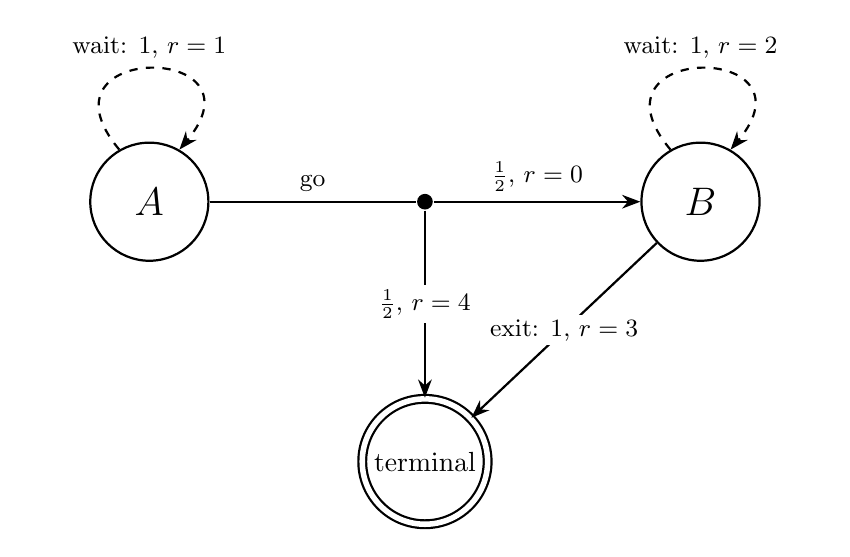
\begin{tikzpicture}[>=Stealth, thick, font=\small,
    st/.style={circle, draw, minimum size=1.5cm, font=\Large},
    lbl/.style={fill=white, inner sep=1.5pt}]
  \node[st] (A) at (0,0) {$A$};
  \node[st] (B) at (7,0) {$B$};
  \node[st, double, double distance=2pt, font=\normalsize] (T) at (3.5,-3.3) {terminal};
  \node[circle, fill, inner sep=2pt] (g) at (3.5,0) {};
  % A: wait (deterministic self-loop)
  \draw[->, dashed] (A.120) to[out=130, in=50, looseness=6] node[above] {wait: $1$, $r=1$} (A.60);
  % A: go (random)
  \draw (A) -- node[above] {go} (g);
  \draw[->] (g) -- node[above] {$\tfrac12$, $r=0$} (B);
  \draw[->] (g) -- node[lbl] {$\tfrac12$, $r=4$} (T);
  % B: wait and exit (deterministic)
  \draw[->, dashed] (B.120) to[out=130, in=50, looseness=6] node[above] {wait: $1$, $r=2$} (B.60);
  \draw[->] (B) -- node[lbl] {exit: $1$, $r=3$} (T);
\end{tikzpicture}
\end{center}

The policy $\pi$ chooses wait and go with probability $\tfrac12$ each at $A$, and always chooses exit at $B$. Every
sweep (i.e. an application of a step of an iterative algorithm) below is \textbf{synchronous}: all new entries use the previous sweep's table. Terminal continuation is always
zero.

\begin{parts}
\part[6] Starting from the expected-return meaning of $\vpi$, write the two Bellman equations for this particular
policy. Show where both the policy probability and the transition probability enter at $A$. Explain why the remaining
return after reaching $B$ can be replaced by $\vpi(B)$. Do not solve the equations.
\begin{solution}
\[
\vpi(A)=\tfrac12\big[1+\tfrac12\vpi(A)\big]+\tfrac12\Big\{\tfrac12\big[0+\tfrac12\vpi(B)\big]+\tfrac12\big[4+\tfrac12\cdot 0\big]\Big\},
\qquad \vpi(B)=3 .
\]
Equivalently $\vpi(A)=\tfrac32+\tfrac14\vpi(A)+\tfrac18\vpi(B)$. The outer $\tfrac12$'s are $\pi(a\mid A)$; the inner
$\tfrac12$'s are the outcome probabilities of go. Given the next state $B$, the Markov property and continued use of
$\pi$ make the expected remaining return $\vpi(B)$.
Rubric: policy averaging 1, wait reward and continuation 1, averaging over go's outcomes 1, go's reward, discount
and terminal handling 1, $B$ equation 1, conditional-return explanation 1. (Exact solution, not required: $(5/2, 3)$.)
\end{solution}
\vfill
\newpage

\part[4] Starting with $V_0(A)=V_0(B)=0$, perform two synchronous policy-evaluation sweeps for $\pi$. Fill in the
table, showing each backup.

\begin{center}
\renewcommand{\arraystretch}{1.2}
\begin{tabular}{|c|c|c|}
\hline
$k$ & $V_k(A)$ & $V_k(B)$ \\ \hline
0 & 0 & 0 \\ \hline
1\cell & \myAnswer{$3/2$} & \myAnswer{$3$} \\ \hline
2\cell & \myAnswer{$9/4$} & \myAnswer{$3$} \\ \hline
\end{tabular}
\end{center}
\begin{solution}
$V_1(A)=\tfrac12(1+0)+\tfrac12\big(\tfrac12\cdot 0+\tfrac12\cdot 4\big)=\tfrac32$, $V_1(B)=3$.
$V_2(A)=\tfrac32+\tfrac14 V_1(A)+\tfrac18 V_1(B)=\tfrac32+\tfrac38+\tfrac38=\tfrac94$, $V_2(B)=3$.
Rubric: 1 per cell (backup from the previous table 0.5, result 0.5). Carry a student's own earlier values forward;
in-place updates keep the method credit but lose the affected result credit.
\end{solution}
\vfill
\newpage

\part[8] Start again from $V_0(A)=V_0(B)=0$. Perform two synchronous \textbf{value-iteration} sweeps, showing both
action-backup values at each state and identifying the maximum. Do not continue the table from part (b).

\begin{center}
\renewcommand{\arraystretch}{1.2}
\begin{tabular}{|c|c|c|c|c|c|c|}
\hline
Sweep & $A$: wait & $A$: go & $V(A)$ & $B$: wait & $B$: exit & $V(B)$ \\ \hline
1\cell & \myAnswer{1} & \myAnswer{2} & \myAnswer{2} & \myAnswer{2} & \myAnswer{3} & \myAnswer{3} \\ \hline
2\cell & \myAnswer{2} & \myAnswer{$11/4$} & \myAnswer{$11/4$} & \myAnswer{$7/2$} & \myAnswer{3} & \myAnswer{$7/2$} \\ \hline
\end{tabular}
\end{center}
\begin{solution}
Sweep 2 from $(2,3)$: $A$ wait $1+\tfrac12\cdot 2=2$; $A$ go $\tfrac12\big(0+\tfrac12\cdot 3\big)+\tfrac12\cdot 4=\tfrac{11}{4}$;
$B$ wait $2+\tfrac12\cdot 3=\tfrac72$; $B$ exit $3$. The maximizing action at $B$ changes from exit to wait.
Rubric: for each state and sweep, both action backups 1 (0.5 each) and the maximum 1; four rows, 8 in total.
\end{solution}
\vfill

\part[8] Independently of parts (b) and (c), the exact values of the original policy are supplied:
$\vpi(A)=\tfrac52$ and $\vpi(B)=3$. Compute $\qpi$ for each of the four state--action pairs. State the greedy improved
policy and check that its selected $\qpi$ value is at least $\vpi$ at each state.
\begin{solution}
$\qpi(A,\text{wait})=1+\tfrac12\cdot\tfrac52=\tfrac94$; $\qpi(A,\text{go})=\tfrac12\big(0+\tfrac12\cdot 3\big)+\tfrac12\cdot 4=\tfrac{11}{4}$;
$\qpi(B,\text{wait})=2+\tfrac12\cdot 3=\tfrac72$; $\qpi(B,\text{exit})=3$ (1 each).
Greedy policy: go at $A$, wait at $B$ (1 each). Checks: $\tfrac{11}{4}\ge\tfrac52$ and $\tfrac72\ge 3$ (1 each). These
are action values under the original $\pi$ after the first action, not the values of the new policy; do not label
them $v^*$.
\end{solution}
\vfill
\newpage

\part[6] Let $\pi'$ be the greedy policy from part (d). Part (d) checks that using $\pi'$ for one step and then
following $\pi$ is at least as good as following $\pi$ throughout: $\vpi(s)\le\qpi(s,\pi'(s))$ at both states. Explain why
using $\pi'$ for two steps and then following $\pi$ is at least as good as using it for one step. (Hint: apply the same
inequality at the state reached after the first step.) What happens as the number of steps using $\pi'$ grows, and what
does this imply about $v^{\pi'}$ and $\vpi$? Then state the main difference between a policy-iteration cycle and a
value-iteration sweep.
\begin{solution}
$\qpi(s,\pi'(s))$ is the expected value of $R_{t+1}+\gamma\vpi(S_{t+1})$ when $\pi'(s)$ is taken. Replacing $\vpi(S_{t+1})$
by $\qpi(S_{t+1},\pi'(S_{t+1}))$ lowers no term (at a terminal successor both continuations are zero), and probabilities and
$\gamma$ are nonnegative, so the average does not fall; the result is two steps of $\pi'$ and then $\pi$. Repeating gives
$k$ steps of $\pi'$ followed by $\pi$, a sequence that never decreases. Values are bounded and the remaining part is
discounted by $\gamma^k\to 0$, so the limit is $v^{\pi'}$ and $v^{\pi'}(s)\ge\vpi(s)$. Here $A$: $\tfrac52,\tfrac{11}{4},\tfrac{23}{8},\ldots\to 3$
and $B$: $3,\tfrac72,\tfrac{15}{4},\ldots\to 4$ (not required).
Policy iteration evaluates a fixed policy (exactly or nearly) and then improves it greedily; value iteration applies
the maximizing backup in every sweep without first completing a fixed-policy evaluation.
Rubric: two-step argument 2 (inequality at each successor 1, averaging preserves it 1), growing $k$ 1, vanishing tail
and conclusion 1, PI 1, VI 1. Accept a verbal argument. Award the reasoning points independently of a mistaken action
choice in (d) when the student correctly uses the supplied inequality.
\end{solution}
\vfill
\newpage

%%%%%%%%%%%%%%%%%%%%%%%%%%%%%%%%%%%%%%%%%%%%%%%%%%%%%%%%%%%%%%%%%%%%%%%%%%%%%%%%%%%%%
% Q4 (ChatGPT Q3a-b with C02 and the added every-visit estimate (D01); Claude Q3e batch part (D03))
\end{parts}
\question (20 points) A fixed policy $\pi$ produced these two complete episodes. Each arrow is labelled by the reward
received on that transition. The model is unknown. Discount $\gamma = \tfrac12$.

\begin{itemize}
  \item Episode 1: $A \xrightarrow{\;0\;} A \xrightarrow{\;2\;} B \xrightarrow{\;4\;}$ terminal
  \item Episode 2: $A \xrightarrow{\;0\;} B \xrightarrow{\;2\;}$ terminal
\end{itemize}
The actions are omitted because this question only evaluates $\pi$.

\begin{parts}
\part[7] Use \textbf{first-visit} Monte Carlo sample averages over both episodes to estimate $V(A)$ and $V(B)$. Then
give the \textbf{every-visit} Monte Carlo estimate of $V(A)$. For each estimate, list the returns you included.
\begin{solution}
Episode 1 returns: $G_2=4$, $G_1=2+\tfrac12\cdot 4=4$, $G_0=0+\tfrac12\cdot 4=2$. Episode 2: $G_1=2$, $G_0=1$.
First-visit: $V(A)=(2+1)/2=\tfrac32$, $V(B)=(4+2)/2=3$. Every-visit: $V(A)=(2+4+1)/3=\tfrac73$ (episode 1's second
visit to $A$ has return 4).
Rubric: first-visit included returns 2, first-visit estimates 2, every-visit included returns for $A$ 1, its estimate
1, correct visit counts 1.
\end{solution}
\vfill

\part[7] Independently of part (a), initialize $V(A)=2$ and $V(B)=0$. With $\alpha=\tfrac12$, apply TD(0) updates
online, in time order, through \textbf{episode 1 only}. For each transition, give the target and the updated value.

\begin{center}
\renewcommand{\arraystretch}{1.2}
\begin{tabular}{|c|c|c|c|}
\hline
Transition & Target $U_t$ & Updated entry & $(V(A), V(B))$ after \\ \hline
$A \xrightarrow{0} A$\cell & \myAnswer{$0+\tfrac12\cdot 2=1$} & \myAnswer{$V(A)=2+\tfrac12(1-2)=\tfrac32$} & \myAnswer{$(\tfrac32, 0)$} \\ \hline
$A \xrightarrow{2} B$\cell & \myAnswer{$2+\tfrac12\cdot 0=2$} & \myAnswer{$V(A)=\tfrac32+\tfrac12(2-\tfrac32)=\tfrac74$} & \myAnswer{$(\tfrac74, 0)$} \\ \hline
$B \xrightarrow{4}$ terminal\cell & \myAnswer{$4$} & \myAnswer{$V(B)=0+\tfrac12(4-0)=2$} & \myAnswer{$(\tfrac74, 2)$} \\ \hline
\end{tabular}
\end{center}
\begin{solution}
The first target and the subtracted estimate both use the pre-update value $V(A)=2$ (self-transition).
Rubric: each target 1, each update from the student's current table 1, chronological use of the reset table 1.
\end{solution}
\vfill
\newpage

\part[6] This part uses \textbf{new data} and $\gamma = 1$. The data are four complete episodes:
\begin{itemize}
  \item twice: $C \xrightarrow{\;+1\;} D \xrightarrow{\;0\;}$ terminal;
  \item twice: $D \xrightarrow{\;+2\;}$ terminal.
\end{itemize}
Using the batch convention from class (repeated passes over this fixed data, increments summed over a pass with the
table held fixed, and a small enough step size to converge), what do batch Monte Carlo and batch TD(0) converge to for
$V(C)$ and $V(D)$? Which answer would you trust if you knew the process was Markov, and why might you doubt that here?
\begin{solution}
Both methods: $V(D)=(0+0+2+2)/4=1$ (1). Batch MC: $V(C)=1$, the mean of its observed returns (1). Batch TD:
$V(C)=1+V(D)=2$ (2). If the process is Markov, TD's answer uses all four outcomes observed from $D$
(certainty equivalence) (1). Here $D$ gave 0 every time it followed $C$ and 2 every time it started an episode, which
hints that ``$D$'' may hide relevant history; then pooling its outcomes can mislead. Two episodes of each kind are
little evidence either way (1). For the ``trust'' point, also credit a reasoned answer that neither estimate is
guaranteed to be more accurate from four episodes. Do not require a claim that the data prove the process is not
Markov.
\end{solution}
\vfill
\newpage

%%%%%%%%%%%%%%%%%%%%%%%%%%%%%%%%%%%%%%%%%%%%%%%%%%%%%%%%%%%%%%%%%%%%%%%%%%%%%%%%%%%%%
% Q5 (ChatGPT Q4)
\end{parts}
\question (14 points) This is a new independent episode, with $\gamma=\tfrac12$ and time indices $0,1,2,3$:
\[
A \xrightarrow{\;2\;} B \xrightarrow{\;0\;} C \xrightarrow{\;4\;} \text{terminal}.
\]
Hold the value table fixed throughout: $V(A)=0$, $V(B)=4$, $V(C)=6$, and terminal value 0. Targets are for the visit
to $A$ at time 0; do not update the table between calculations.

\begin{parts}
\part[4] Expand the return recursion twice and replace the unobserved return after the second transition with its
value estimate. Write the resulting two-step target $G_{0:2}$ symbolically before inserting numbers.
\begin{solution}
$G_0=R_1+\gamma G_1=R_1+\gamma R_2+\gamma^2 G_2$; replacing $G_2$ with $V(S_2)$ gives
$G_{0:2}=R_1+\gamma R_2+\gamma^2 V(S_2)$.
Rubric: first expansion 1, second expansion with correct discount powers 1, replacement at the second successor 1,
correct target 1.
\end{solution}
\vfill

\part[6] Calculate the one-step target $G_{0:1}$, the two-step target $G_{0:2}$ and the full return $G_0$. For the
full return, indicate why there is no additional bootstrap term.
\begin{solution}
$G_{0:1}=2+\tfrac12\cdot 4=4$. $G_{0:2}=2+\tfrac12\cdot 0+\tfrac14\cdot 6=\tfrac72$.
$G_0=2+\tfrac12\cdot 0+\tfrac14\cdot 4=3$: the episode ended, so there is no continuation to bootstrap from.
Rubric: each target, expression 1 and result 1.
\end{solution}
\vfill
\newpage

\part[1] If this episode arrives one transition at a time, at which time index does the two-step target for $A$ first
become available? Must the learner wait until termination here?
\begin{solution}
At time 2, after observing $R_2=0$ and $S_2=C$; no need to wait for termination at time 3.
\end{solution}
\vfill

\part[3] A student sets $\lambda=1$ in the finite episodic forward $\lambda$-return to remove bootstrapping, then
concludes that the target must be more accurate than TD(0). Assess both claims briefly.
\begin{solution}
At $\lambda=1$ the $\lambda$-return is the complete return and does not bootstrap (1). The accuracy claim is false (1):
removing the table from the target does not remove sampling variability, so the error need not be lower and a good
bootstrapped estimate can help (1).
\end{solution}
\vfill
\end{parts}

%%%%%%%%%%%%%%%%%%%%%%%%%%%%%%%%%%%%%%%%%%%%%%%%%%%%%%%%%%%%%%%%%%%%%%%%%%%%%%%%%%%%%
% Equation sheet (ChatGPT's sheet with C03 (i)-(ii); finite lambda-return included under X1)
\newpage
Several Equations (semantics and context are not given on purpose)

\begin{align*}
G_t &= \sum_{k=0}^{T-t-1}\gamma^{k}R_{t+k+1}, \qquad G_t = R_{t+1}+\gamma G_{t+1}, \qquad G_T = 0 \\[4pt]
\vpi(s) &= \E_\pi[G_t\mid S_t=s], \qquad \qpi(s,a) = \E_\pi[G_t\mid S_t=s, A_t=a] \\[4pt]
\vpi(s) &= \sum_a \pi(a\mid s)\,\qpi(s,a) \\[4pt]
\qpi(s,a) &= \sum_{s',r}\M(s,a,r,s')\big[r+\gamma\,\vpi(s')\big] \\[4pt]
v^*(s) &= \max_a \sum_{s',r}\M(s,a,r,s')\big[r+\gamma\,v^*(s')\big], \qquad \pi^*(s)\in\argmax_a q^*(s,a) \\[4pt]
V_{k+1}(s) &= \sum_a \pi(a\mid s)\sum_{s',r}\M(s,a,r,s')\big[r+\gamma\,V_k(s')\big] \\[4pt]
V_{k+1}(s) &= \max_a \sum_{s',r}\M(s,a,r,s')\big[r+\gamma\,V_k(s')\big] \\[4pt]
V(S_t) &\leftarrow V(S_t)+\alpha\big[U_t-V(S_t)\big] \\[4pt]
U_t &= G_t, \qquad U_t = R_{t+1}+\gamma V(S_{t+1}) \\[4pt]
V(s) &\leftarrow V(s)+\frac{1}{N(s)}\big[G_t-V(s)\big], \qquad S_t=s \\[4pt]
G_t^{\lambda} &= (1-\lambda)\sum_{n=1}^{T-t-1}\lambda^{n-1}G_{t:t+n}+\lambda^{T-t-1}G_t, \qquad 0\le\lambda\le 1,\quad t<T
\end{align*}

\end{questions}

\end{document}
"
%
% Exam Template for UMTYMP and Math Department courses
%
% Using Philip Hirschhorn's exam.cls: http://www-math.mit.edu/~psh/#ExamCls
%
% run pdflatex on a finished exam at least three times to do the grading table on front page.
%
%%%%%%%%%%%%%%%%%%%%%%%%%%%%%%%%%%%%%%%%%%%%%%%%%%%%%%%%%%%%%%%%%%%%%%%%%%%%%%%%%%%%%%%%%%%%%%

\documentclass[11pt]{exam}
\RequirePackage{amssymb, amsfonts, amsmath, latexsym, verbatim, xspace, setspace}
\RequirePackage{tikz, pgflibraryplotmarks}
\usetikzlibrary{arrows.meta}

\usepackage[margin=2.1cm]{geometry}
\usepackage[utf8]{inputenc}
\usepackage[english]{babel}
\usepackage{wrapfig}
\usepackage{textpos}
\usepackage{tabularx}
\usepackage{color}
\usepackage{ulem}
\usepackage{multirow}
\usepackage{enumitem}
\usepackage{multicol}
\usepackage{graphicx}
\usepackage{subcaption}
\usepackage{bbm}
\usepackage[T1]{fontenc}
\usepackage{changepage}

\usepackage{amsmath}
\DeclareMathOperator*{\argmax}{arg\,max}
\DeclareMathOperator*{\argmin}{arg\,min}

\definecolor{red}{rgb}{1.0,0.0,0.0}
\definecolor{green}{rgb}{0.0,1.0,0.0}
\definecolor{blue}{rgb}{0.0,0.0,1.0}

\newif\ifexternal
%\externaltrue

\newif\ifonline
\onlinefalse

% Answers are printed only when \withsolutions is defined (see the build lines at the top).
\ifdefined\withsolutions \printanswers \fi
\newcommand{\myAnswer}[1]{\ifprintanswers {\color{blue}#1} \fi}
\newcommand{\myAB}[2]{\ifprintanswers {\color{blue}#1} \else #1 \fi}
\newcommand{\myBlank}[1]{\ifprintanswers {\color{blue}#1} \else \hphantom{#1} \fi}

\SolutionEmphasis{\color{blue}}
\unframedsolutions

% Here's where you edit the Class, Exam, Date, etc.
\newcommand{\class}{COMP 438/538}
\newcommand{\classname}{COMP 438/538: INTRODUCTION TO REINFORCEMENT LEARNING}
\newcommand{\term}{Fall 2026}
\newcommand{\examnum}{MT1}
\newcommand{\examname}{Midterm 1}

\newcommand{\examdate}{05/11/2026}
\newcommand{\timelimit}{100 Minutes}
\newcommand{\instructor}{Bar\i\c{s} Akg\"un}

% Course notation (course/notation_guide.md)
\newcommand{\M}{\mathcal{M}}
\newcommand{\E}{\mathbb{E}}
\newcommand{\vpi}{v^{\pi}}
\newcommand{\qpi}{q^{\pi}}
\newcommand{\cell}{\rule{0pt}{1.1cm}}

\parindent 0ex

\newcolumntype{L}{>{\raggedright\arraybackslash}X}%
\newcolumntype{R}{>{\raggedleft\arraybackslash}X}%
\newcolumntype{C}{>{\centering\arraybackslash}X}

\setlength{\abovedisplayskip}{4pt}
\setlength{\belowdisplayskip}{4pt}
\setlength{\abovedisplayshortskip}{2pt}
\setlength{\belowdisplayshortskip}{2pt}

\begin{document}

  \begin{center}
    {\scshape\Large KO\c{C} UNIVERSITY \par}
    {\scshape\Large College of Engineering\par}
    \vspace{0.5cm}
    {\LARGE\bfseries \classname \par}
    \vspace{0.5cm}
    {\scshape\Large \bfseries \examname \par}
    {\scshape\large \term, \examdate \par}
    {\scshape\large Duration: \timelimit  \par}
    \vspace{0.3cm}
    \hrulefill
    \vspace{0.2cm}
  \end{center}

    \begin{tabular}{l l}
      \textbf{Name:} & \makebox[10cm]{\uline{ \myAnswer{Solutions} \hfill }}   \\
      & \\
      \textbf{ID:} & \makebox[10cm]{\uline{ \myAnswer{00110001 00110000 00110000} \hfill }}
    \end{tabular}

  \vspace{0.4cm}
  \hrulefill
\begin{center}
{\large \bfseries Read These Instructions Carefully}
\end{center}
\begin{itemize}
  \item This exam contains \numpages\ pages including this cover page and \numquestions\ questions. Check to see if any
  pages are missing. Put your initials on the top of every page, in case the pages become separated.
  \item  By submitting this exam, you \textbf{agree} to fully comply with Ko\c{c} University Student Code of Conduct,
  and accept any punishment in case of failure to comply. If you do not submit this exam on time, you will receive 0 credits.
  \item The exam is \textbf{closed book} and \textbf{closed notes}. You are \textbf{not} allowed to use any additional
  material including any electronic equipment such as computers and  mobile phones. An equation sheet is provided on
  the last page.
  \item You are expected to be able to provide clear and concise answers. Gibberish will not receive any credit. Your answers need to be readable by a human,
  illegible writing is not gradable.
  \item Show the essential calculations or a short justification. Exact fractions or equivalent decimals are acceptable.
  Each question describes a separate problem; state names are local to their question. Terminal states have zero
  continuation value, and a reward shown on a transition is the total reward for that transition.
  \item Read each question \uline{carefully} and make sure to follow instructions. The written instructions take
  precedence over an answer that the instructor might give you during the exam, unless the instructor makes a class-wide announcement.
  \item Do not write in the table below.
\end{itemize}

\hrulefill
  \begin{center}
    \vspace{0.2cm}
    \gradetablestretch{1.8}
    \vqword{Question}
    \addpoints
    \gradetable[h]
  \end{center}

\newpage % End of cover page
\runningheader{\class}{\examnum\ - Page \thepage\ of \numpages}{\examdate}
\runningheadrule

\begin{questions}

%%%%%%%%%%%%%%%%%%%%%%%%%%%%%%%%%%%%%%%%%%%%%%%%%%%%%%%%%%%%%%%%%%%%%%%%%%%%%%%%%%%%%
% Q1: short answers, placed first as a warm-up (instructor, 2026-11-03). Was Q5: ChatGPT Q5a, Q5b (X8);
% Claude T/F 3 true form, 4, 5.
\question (12 points) Short answers.

\begin{parts}
\part[2] Consider two policies for a continuing service task. One produces reward 0.75 every step. The other repeats
the rewards $0, 2, 0, 2, \ldots$ forever. Which has the higher long-run average reward per step, and why? No
average-reward learning algorithm is required.
\begin{solution}
The alternating policy: $(0+2)/2=1$ per step versus 0.75 (1 for the rates, 1 for the comparison).
\end{solution}
\vfill

\part[4] A report compares MC and TD prediction on a fixed policy. It tries many step sizes and selects each method's
best setting using the same episodes and seeds on which it reports final value error. It then uses the single
lowest-error run to claim that the selected method is generally better. Identify two weaknesses and suggest a fix for each. 
No statistical test or numerical uncertainty calculation is required.
\begin{solution}
(1) Settings were chosen on the runs used for the reported result, so the result is optimistic; repair: choose
settings on separate development runs, then report fresh final runs at those settings. (2) One best run does not show
typical performance; repair: run many independent runs and report the mean error with its variability, not the best
seed. Rubric: 1 per weakness, 1 per repair. A fair-budget answer earns credit only if it is tied to one of these flaws.
\end{solution}
\vfill
\newpage

\uplevel{For each statement below, write \textbf{True} or \textbf{False} and give a one-line justification. Each is
worth 2 points: 1 for the verdict and 1 for the justification. A verdict without a justification receives 0.}

\part[2] Given $q^*$, a greedy optimal policy can be obtained without the model, however, obtaining one from $v^*$ by one-step
lookahead needs the model.
\begin{solution}
True: $\argmax_a q^*(s,a)$ needs no model; with $v^*$, comparing actions needs the expected rewards and transition
probabilities.
\end{solution}
\vfill

\part[2] If the current policy is not optimal, one greedy policy-improvement step using its exact action values
increases the value of at least one nonterminal state.
\begin{solution}
True: a suboptimal policy must admit a strict one-step gain somewhere; otherwise $\vpi(s)=\max_a\qpi(s,a)$ at every
state, which is the Bellman optimality equation. By the policy improvement theorem the greedy policy keeps that gain
and lowers no state. Rubric: verdict 1, reason for the strict gain 1, in ordinary language. Naming the policy
improvement theorem without that reason earns 0.5 of the reason point; a change of action at a tie alone earns none.
\end{solution}
\vfill

\part[2] The Monte Carlo prediction method we used in class can be applied directly to a continuing task that never
terminates.
\begin{solution}
False: the method waits for a finished episode to observe its target, so without termination it never gets one.
Rubric: verdict 1, reason 1. Full credit for explaining that a finite cutoff would change the target; ``True, by
truncating'' earns no verdict point. Mentioning TD is not required.
\end{solution}
\vfill

\end{parts}
\newpage

%%%%%%%%%%%%%%%%%%%%%%%%%%%%%%%%%%%%%%%%%%%%%%%%%%%%%%%%%%%%%%%%%%%%%%%%%%%%%%%%%%%%%
% Q2 (Claude Q1 with review wording R01-R03). Partial credit for alternative answers: instructor (X6).
\question (22 points) An online tutoring app runs a practice session of exactly 20 questions. Before each question it
chooses a difficulty: easy, medium or hard. After each question it sees only whether the answer was correct and how
many seconds it took. The student's actual skill is not visible, and it changes as the student practises. After the
20th question the student takes a fixed 10-question test that the app does not choose.

The designer's objective is to maximize the student's expected score on the fixed final test. No model of how
difficulty affects skill, correctness or response time is supplied.

\begin{parts}
\part[4] What are the actions? What does the app observe after each question?
\begin{solution}
Actions: easy, medium, hard (2). Observation after each question: whether the answer was correct and the response
time (2). Additional observed features (e.g.\ the topic) are fine if justified.
\end{solution}
\vfill

\part[6] Explain why the latest observation alone need not be a Markov state. Give two plausible histories ending in
the same observation that could suggest different skill levels. Propose a history-based agent state for choosing the
next difficulty, justify the information you retain, and mention one limitation. A justified approximation is
sufficient; you do not need to prove that it is Markov.
\begin{solution}
The skill is hidden and changes, so the latest answer alone does not summarize what matters for the next outcome (1).
Example: ``correct, 20 seconds'' after ten correct hard answers versus after ten wrong easy answers suggests very
different skill and a different next difficulty (2). Example agent state $S_t = f(H_t)$: recent counts of correct
answers per difficulty (or an estimated skill level), plus questions remaining (2). Justification and one limitation,
e.g.\ counts discard the order of answers, so improvement over the session can be missed (1).
\end{solution}
\vfill
\newpage

\part[6] Designer A rewards each correct practice answer with $+1$ and gives $0$ otherwise. Designer B gives the final
test score ($0$--$10$) after the session and $0$ otherwise. Describe a plausible way A could encourage behaviour that
does not improve the final test score. Which reward more directly matches the stated objective, and what makes
learning from it difficult? You do not need to identify an optimal sequence of difficulties.
\begin{solution}
A can encourage choosing easy questions for immediate correct answers even when harder practice would teach more: an
incentive mismatch, not a claim about the optimal policy for every student (2). B rewards the stated objective
directly (2), but the feedback is delayed and sparse: one number after 20 decisions, so assigning credit to
individual difficulty choices is hard and many sessions are needed (2).
\end{solution}
\vfill

\part[4] Is the task episodic or continuing? Should the number of questions remaining be part of the agent state? Why?
\begin{solution}
Episodic: the session ends after 20 questions and the test (1). Yes (1): with a deadline, the best difficulty can
depend on the time left, e.g.\ hard practice may pay off only if enough practice follows, so the same skill estimate
with 2 or 15 questions left can call for different actions (2). The ``Yes'' point does not require a separate
counter: a state that already contains the remaining number of questions, e.g.\ the full history or the elapsed
number of questions, earns it.
\end{solution}
\vfill

\part[2] With no model of the student's responses or learning dynamics supplied, can you directly apply ordinary
tabular value iteration to compute a policy? What information would be needed?
\begin{solution}
No (1): value iteration needs the expected rewards and next-state probabilities for a usable Markov state, which are
not provided; experience, or an independently supplied model, would be needed (1). A conditional answer (``with a
usable Markov model, yes'') earns full credit.
\end{solution}
\vfill
\newpage

%%%%%%%%%%%%%%%%%%%%%%%%%%%%%%%%%%%%%%%%%%%%%%%%%%%%%%%%%%%%%%%%%%%%%%%%%%%%%%%%%%%%%
% Q3 (ChatGPT Q2; Q3b 4 points under X8; model figure replaces the table, instructor 2026-11-03)
\end{parts}
\question (32 points) There are two nonterminal states $A$ and $B$, and a terminal state. The discount is
$\gamma = \tfrac12$. The figure shows every possible transition. The black dot shows the possible outcomes after choosing go. Each arrow
gives the probability $\M(s,a,r,s')$ and the reward $r$ of its outcome. All other outcomes have probability zero.

\begin{center}
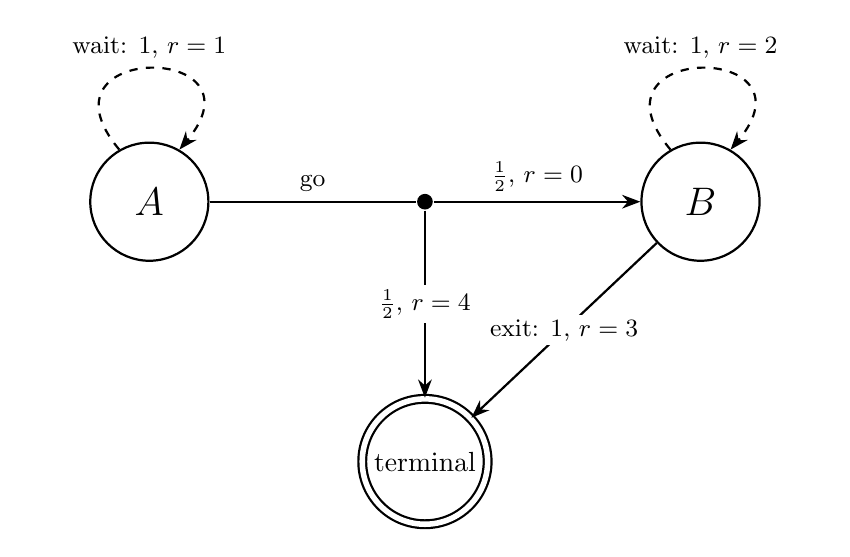
\begin{tikzpicture}[>=Stealth, thick, font=\small,
    st/.style={circle, draw, minimum size=1.5cm, font=\Large},
    lbl/.style={fill=white, inner sep=1.5pt}]
  \node[st] (A) at (0,0) {$A$};
  \node[st] (B) at (7,0) {$B$};
  \node[st, double, double distance=2pt, font=\normalsize] (T) at (3.5,-3.3) {terminal};
  \node[circle, fill, inner sep=2pt] (g) at (3.5,0) {};
  % A: wait (deterministic self-loop)
  \draw[->, dashed] (A.120) to[out=130, in=50, looseness=6] node[above] {wait: $1$, $r=1$} (A.60);
  % A: go (random)
  \draw (A) -- node[above] {go} (g);
  \draw[->] (g) -- node[above] {$\tfrac12$, $r=0$} (B);
  \draw[->] (g) -- node[lbl] {$\tfrac12$, $r=4$} (T);
  % B: wait and exit (deterministic)
  \draw[->, dashed] (B.120) to[out=130, in=50, looseness=6] node[above] {wait: $1$, $r=2$} (B.60);
  \draw[->] (B) -- node[lbl] {exit: $1$, $r=3$} (T);
\end{tikzpicture}
\end{center}

The policy $\pi$ chooses wait and go with probability $\tfrac12$ each at $A$, and always chooses exit at $B$. Every
sweep (i.e. an application of a step of an iterative algorithm) below is \textbf{synchronous}: all new entries use the previous sweep's table. Terminal continuation is always
zero.

\begin{parts}
\part[6] Starting from the expected-return meaning of $\vpi$, write the two Bellman equations for this particular
policy. Show where both the policy probability and the transition probability enter at $A$. Explain why the remaining
return after reaching $B$ can be replaced by $\vpi(B)$. Do not solve the equations.
\begin{solution}
\[
\vpi(A)=\tfrac12\big[1+\tfrac12\vpi(A)\big]+\tfrac12\Big\{\tfrac12\big[0+\tfrac12\vpi(B)\big]+\tfrac12\big[4+\tfrac12\cdot 0\big]\Big\},
\qquad \vpi(B)=3 .
\]
Equivalently $\vpi(A)=\tfrac32+\tfrac14\vpi(A)+\tfrac18\vpi(B)$. The outer $\tfrac12$'s are $\pi(a\mid A)$; the inner
$\tfrac12$'s are the outcome probabilities of go. Given the next state $B$, the Markov property and continued use of
$\pi$ make the expected remaining return $\vpi(B)$.
Rubric: policy averaging 1, wait reward and continuation 1, averaging over go's outcomes 1, go's reward, discount
and terminal handling 1, $B$ equation 1, conditional-return explanation 1. (Exact solution, not required: $(5/2, 3)$.)
\end{solution}
\vfill
\newpage

\part[4] Starting with $V_0(A)=V_0(B)=0$, perform two synchronous policy-evaluation sweeps for $\pi$. Fill in the
table, showing each backup.

\begin{center}
\renewcommand{\arraystretch}{1.2}
\begin{tabular}{|c|c|c|}
\hline
$k$ & $V_k(A)$ & $V_k(B)$ \\ \hline
0 & 0 & 0 \\ \hline
1\cell & \myAnswer{$3/2$} & \myAnswer{$3$} \\ \hline
2\cell & \myAnswer{$9/4$} & \myAnswer{$3$} \\ \hline
\end{tabular}
\end{center}
\begin{solution}
$V_1(A)=\tfrac12(1+0)+\tfrac12\big(\tfrac12\cdot 0+\tfrac12\cdot 4\big)=\tfrac32$, $V_1(B)=3$.
$V_2(A)=\tfrac32+\tfrac14 V_1(A)+\tfrac18 V_1(B)=\tfrac32+\tfrac38+\tfrac38=\tfrac94$, $V_2(B)=3$.
Rubric: 1 per cell (backup from the previous table 0.5, result 0.5). Carry a student's own earlier values forward;
in-place updates keep the method credit but lose the affected result credit.
\end{solution}
\vfill
\newpage

\part[8] Start again from $V_0(A)=V_0(B)=0$. Perform two synchronous \textbf{value-iteration} sweeps, showing both
action-backup values at each state and identifying the maximum. Do not continue the table from part (b).

\begin{center}
\renewcommand{\arraystretch}{1.2}
\begin{tabular}{|c|c|c|c|c|c|c|}
\hline
Sweep & $A$: wait & $A$: go & $V(A)$ & $B$: wait & $B$: exit & $V(B)$ \\ \hline
1\cell & \myAnswer{1} & \myAnswer{2} & \myAnswer{2} & \myAnswer{2} & \myAnswer{3} & \myAnswer{3} \\ \hline
2\cell & \myAnswer{2} & \myAnswer{$11/4$} & \myAnswer{$11/4$} & \myAnswer{$7/2$} & \myAnswer{3} & \myAnswer{$7/2$} \\ \hline
\end{tabular}
\end{center}
\begin{solution}
Sweep 2 from $(2,3)$: $A$ wait $1+\tfrac12\cdot 2=2$; $A$ go $\tfrac12\big(0+\tfrac12\cdot 3\big)+\tfrac12\cdot 4=\tfrac{11}{4}$;
$B$ wait $2+\tfrac12\cdot 3=\tfrac72$; $B$ exit $3$. The maximizing action at $B$ changes from exit to wait.
Rubric: for each state and sweep, both action backups 1 (0.5 each) and the maximum 1; four rows, 8 in total.
\end{solution}
\vfill

\part[8] Independently of parts (b) and (c), the exact values of the original policy are supplied:
$\vpi(A)=\tfrac52$ and $\vpi(B)=3$. Compute $\qpi$ for each of the four state--action pairs. State the greedy improved
policy and check that its selected $\qpi$ value is at least $\vpi$ at each state.
\begin{solution}
$\qpi(A,\text{wait})=1+\tfrac12\cdot\tfrac52=\tfrac94$; $\qpi(A,\text{go})=\tfrac12\big(0+\tfrac12\cdot 3\big)+\tfrac12\cdot 4=\tfrac{11}{4}$;
$\qpi(B,\text{wait})=2+\tfrac12\cdot 3=\tfrac72$; $\qpi(B,\text{exit})=3$ (1 each).
Greedy policy: go at $A$, wait at $B$ (1 each). Checks: $\tfrac{11}{4}\ge\tfrac52$ and $\tfrac72\ge 3$ (1 each). These
are action values under the original $\pi$ after the first action, not the values of the new policy; do not label
them $v^*$.
\end{solution}
\vfill
\newpage

\part[6] Let $\pi'$ be the greedy policy from part (d). Part (d) checks that using $\pi'$ for one step and then
following $\pi$ is at least as good as following $\pi$ throughout: $\vpi(s)\le\qpi(s,\pi'(s))$ at both states. Explain why
using $\pi'$ for two steps and then following $\pi$ is at least as good as using it for one step. (Hint: apply the same
inequality at the state reached after the first step.) What happens as the number of steps using $\pi'$ grows, and what
does this imply about $v^{\pi'}$ and $\vpi$? Then state the main difference between a policy-iteration cycle and a
value-iteration sweep.
\begin{solution}
$\qpi(s,\pi'(s))$ is the expected value of $R_{t+1}+\gamma\vpi(S_{t+1})$ when $\pi'(s)$ is taken. Replacing $\vpi(S_{t+1})$
by $\qpi(S_{t+1},\pi'(S_{t+1}))$ lowers no term (at a terminal successor both continuations are zero), and probabilities and
$\gamma$ are nonnegative, so the average does not fall; the result is two steps of $\pi'$ and then $\pi$. Repeating gives
$k$ steps of $\pi'$ followed by $\pi$, a sequence that never decreases. Values are bounded and the remaining part is
discounted by $\gamma^k\to 0$, so the limit is $v^{\pi'}$ and $v^{\pi'}(s)\ge\vpi(s)$. Here $A$: $\tfrac52,\tfrac{11}{4},\tfrac{23}{8},\ldots\to 3$
and $B$: $3,\tfrac72,\tfrac{15}{4},\ldots\to 4$ (not required).
Policy iteration evaluates a fixed policy (exactly or nearly) and then improves it greedily; value iteration applies
the maximizing backup in every sweep without first completing a fixed-policy evaluation.
Rubric: two-step argument 2 (inequality at each successor 1, averaging preserves it 1), growing $k$ 1, vanishing tail
and conclusion 1, PI 1, VI 1. Accept a verbal argument. Award the reasoning points independently of a mistaken action
choice in (d) when the student correctly uses the supplied inequality.
\end{solution}
\vfill
\newpage

%%%%%%%%%%%%%%%%%%%%%%%%%%%%%%%%%%%%%%%%%%%%%%%%%%%%%%%%%%%%%%%%%%%%%%%%%%%%%%%%%%%%%
% Q4 (ChatGPT Q3a-b with C02 and the added every-visit estimate (D01); Claude Q3e batch part (D03))
\end{parts}
\question (20 points) A fixed policy $\pi$ produced these two complete episodes. Each arrow is labelled by the reward
received on that transition. The model is unknown. Discount $\gamma = \tfrac12$.

\begin{itemize}
  \item Episode 1: $A \xrightarrow{\;0\;} A \xrightarrow{\;2\;} B \xrightarrow{\;4\;}$ terminal
  \item Episode 2: $A \xrightarrow{\;0\;} B \xrightarrow{\;2\;}$ terminal
\end{itemize}
The actions are omitted because this question only evaluates $\pi$.

\begin{parts}
\part[7] Use \textbf{first-visit} Monte Carlo sample averages over both episodes to estimate $V(A)$ and $V(B)$. Then
give the \textbf{every-visit} Monte Carlo estimate of $V(A)$. For each estimate, list the returns you included.
\begin{solution}
Episode 1 returns: $G_2=4$, $G_1=2+\tfrac12\cdot 4=4$, $G_0=0+\tfrac12\cdot 4=2$. Episode 2: $G_1=2$, $G_0=1$.
First-visit: $V(A)=(2+1)/2=\tfrac32$, $V(B)=(4+2)/2=3$. Every-visit: $V(A)=(2+4+1)/3=\tfrac73$ (episode 1's second
visit to $A$ has return 4).
Rubric: first-visit included returns 2, first-visit estimates 2, every-visit included returns for $A$ 1, its estimate
1, correct visit counts 1.
\end{solution}
\vfill

\part[7] Independently of part (a), initialize $V(A)=2$ and $V(B)=0$. With $\alpha=\tfrac12$, apply TD(0) updates
online, in time order, through \textbf{episode 1 only}. For each transition, give the target and the updated value.

\begin{center}
\renewcommand{\arraystretch}{1.2}
\begin{tabular}{|c|c|c|c|}
\hline
Transition & Target $U_t$ & Updated entry & $(V(A), V(B))$ after \\ \hline
$A \xrightarrow{0} A$\cell & \myAnswer{$0+\tfrac12\cdot 2=1$} & \myAnswer{$V(A)=2+\tfrac12(1-2)=\tfrac32$} & \myAnswer{$(\tfrac32, 0)$} \\ \hline
$A \xrightarrow{2} B$\cell & \myAnswer{$2+\tfrac12\cdot 0=2$} & \myAnswer{$V(A)=\tfrac32+\tfrac12(2-\tfrac32)=\tfrac74$} & \myAnswer{$(\tfrac74, 0)$} \\ \hline
$B \xrightarrow{4}$ terminal\cell & \myAnswer{$4$} & \myAnswer{$V(B)=0+\tfrac12(4-0)=2$} & \myAnswer{$(\tfrac74, 2)$} \\ \hline
\end{tabular}
\end{center}
\begin{solution}
The first target and the subtracted estimate both use the pre-update value $V(A)=2$ (self-transition).
Rubric: each target 1, each update from the student's current table 1, chronological use of the reset table 1.
\end{solution}
\vfill
\newpage

\part[6] This part uses \textbf{new data} and $\gamma = 1$. The data are four complete episodes:
\begin{itemize}
  \item twice: $C \xrightarrow{\;+1\;} D \xrightarrow{\;0\;}$ terminal;
  \item twice: $D \xrightarrow{\;+2\;}$ terminal.
\end{itemize}
Using the batch convention from class (repeated passes over this fixed data, increments summed over a pass with the
table held fixed, and a small enough step size to converge), what do batch Monte Carlo and batch TD(0) converge to for
$V(C)$ and $V(D)$? Which answer would you trust if you knew the process was Markov, and why might you doubt that here?
\begin{solution}
Both methods: $V(D)=(0+0+2+2)/4=1$ (1). Batch MC: $V(C)=1$, the mean of its observed returns (1). Batch TD:
$V(C)=1+V(D)=2$ (2). If the process is Markov, TD's answer uses all four outcomes observed from $D$
(certainty equivalence) (1). Here $D$ gave 0 every time it followed $C$ and 2 every time it started an episode, which
hints that ``$D$'' may hide relevant history; then pooling its outcomes can mislead. Two episodes of each kind are
little evidence either way (1). For the ``trust'' point, also credit a reasoned answer that neither estimate is
guaranteed to be more accurate from four episodes. Do not require a claim that the data prove the process is not
Markov.
\end{solution}
\vfill
\newpage

%%%%%%%%%%%%%%%%%%%%%%%%%%%%%%%%%%%%%%%%%%%%%%%%%%%%%%%%%%%%%%%%%%%%%%%%%%%%%%%%%%%%%
% Q5 (ChatGPT Q4)
\end{parts}
\question (14 points) This is a new independent episode, with $\gamma=\tfrac12$ and time indices $0,1,2,3$:
\[
A \xrightarrow{\;2\;} B \xrightarrow{\;0\;} C \xrightarrow{\;4\;} \text{terminal}.
\]
Hold the value table fixed throughout: $V(A)=0$, $V(B)=4$, $V(C)=6$, and terminal value 0. Targets are for the visit
to $A$ at time 0; do not update the table between calculations.

\begin{parts}
\part[4] Expand the return recursion twice and replace the unobserved return after the second transition with its
value estimate. Write the resulting two-step target $G_{0:2}$ symbolically before inserting numbers.
\begin{solution}
$G_0=R_1+\gamma G_1=R_1+\gamma R_2+\gamma^2 G_2$; replacing $G_2$ with $V(S_2)$ gives
$G_{0:2}=R_1+\gamma R_2+\gamma^2 V(S_2)$.
Rubric: first expansion 1, second expansion with correct discount powers 1, replacement at the second successor 1,
correct target 1.
\end{solution}
\vfill

\part[6] Calculate the one-step target $G_{0:1}$, the two-step target $G_{0:2}$ and the full return $G_0$. For the
full return, indicate why there is no additional bootstrap term.
\begin{solution}
$G_{0:1}=2+\tfrac12\cdot 4=4$. $G_{0:2}=2+\tfrac12\cdot 0+\tfrac14\cdot 6=\tfrac72$.
$G_0=2+\tfrac12\cdot 0+\tfrac14\cdot 4=3$: the episode ended, so there is no continuation to bootstrap from.
Rubric: each target, expression 1 and result 1.
\end{solution}
\vfill
\newpage

\part[1] If this episode arrives one transition at a time, at which time index does the two-step target for $A$ first
become available? Must the learner wait until termination here?
\begin{solution}
At time 2, after observing $R_2=0$ and $S_2=C$; no need to wait for termination at time 3.
\end{solution}
\vfill

\part[3] A student sets $\lambda=1$ in the finite episodic forward $\lambda$-return to remove bootstrapping, then
concludes that the target must be more accurate than TD(0). Assess both claims briefly.
\begin{solution}
At $\lambda=1$ the $\lambda$-return is the complete return and does not bootstrap (1). The accuracy claim is false (1):
removing the table from the target does not remove sampling variability, so the error need not be lower and a good
bootstrapped estimate can help (1).
\end{solution}
\vfill
\end{parts}

%%%%%%%%%%%%%%%%%%%%%%%%%%%%%%%%%%%%%%%%%%%%%%%%%%%%%%%%%%%%%%%%%%%%%%%%%%%%%%%%%%%%%
% Equation sheet (ChatGPT's sheet with C03 (i)-(ii); finite lambda-return included under X1)
\newpage
Several Equations (semantics and context are not given on purpose)

\begin{align*}
G_t &= \sum_{k=0}^{T-t-1}\gamma^{k}R_{t+k+1}, \qquad G_t = R_{t+1}+\gamma G_{t+1}, \qquad G_T = 0 \\[4pt]
\vpi(s) &= \E_\pi[G_t\mid S_t=s], \qquad \qpi(s,a) = \E_\pi[G_t\mid S_t=s, A_t=a] \\[4pt]
\vpi(s) &= \sum_a \pi(a\mid s)\,\qpi(s,a) \\[4pt]
\qpi(s,a) &= \sum_{s',r}\M(s,a,r,s')\big[r+\gamma\,\vpi(s')\big] \\[4pt]
v^*(s) &= \max_a \sum_{s',r}\M(s,a,r,s')\big[r+\gamma\,v^*(s')\big], \qquad \pi^*(s)\in\argmax_a q^*(s,a) \\[4pt]
V_{k+1}(s) &= \sum_a \pi(a\mid s)\sum_{s',r}\M(s,a,r,s')\big[r+\gamma\,V_k(s')\big] \\[4pt]
V_{k+1}(s) &= \max_a \sum_{s',r}\M(s,a,r,s')\big[r+\gamma\,V_k(s')\big] \\[4pt]
V(S_t) &\leftarrow V(S_t)+\alpha\big[U_t-V(S_t)\big] \\[4pt]
U_t &= G_t, \qquad U_t = R_{t+1}+\gamma V(S_{t+1}) \\[4pt]
V(s) &\leftarrow V(s)+\frac{1}{N(s)}\big[G_t-V(s)\big], \qquad S_t=s \\[4pt]
G_t^{\lambda} &= (1-\lambda)\sum_{n=1}^{T-t-1}\lambda^{n-1}G_{t:t+n}+\lambda^{T-t-1}G_t, \qquad 0\le\lambda\le 1,\quad t<T
\end{align*}

\end{questions}

\end{document}
"
%
% Exam Template for UMTYMP and Math Department courses
%
% Using Philip Hirschhorn's exam.cls: http://www-math.mit.edu/~psh/#ExamCls
%
% run pdflatex on a finished exam at least three times to do the grading table on front page.
%
%%%%%%%%%%%%%%%%%%%%%%%%%%%%%%%%%%%%%%%%%%%%%%%%%%%%%%%%%%%%%%%%%%%%%%%%%%%%%%%%%%%%%%%%%%%%%%

\documentclass[11pt]{exam}
\RequirePackage{amssymb, amsfonts, amsmath, latexsym, verbatim, xspace, setspace}
\RequirePackage{tikz, pgflibraryplotmarks}
\usetikzlibrary{arrows.meta}

\usepackage[margin=2.1cm]{geometry}
\usepackage[utf8]{inputenc}
\usepackage[english]{babel}
\usepackage{wrapfig}
\usepackage{textpos}
\usepackage{tabularx}
\usepackage{color}
\usepackage{ulem}
\usepackage{multirow}
\usepackage{enumitem}
\usepackage{multicol}
\usepackage{graphicx}
\usepackage{subcaption}
\usepackage{bbm}
\usepackage[T1]{fontenc}
\usepackage{changepage}

\usepackage{amsmath}
\DeclareMathOperator*{\argmax}{arg\,max}
\DeclareMathOperator*{\argmin}{arg\,min}

\definecolor{red}{rgb}{1.0,0.0,0.0}
\definecolor{green}{rgb}{0.0,1.0,0.0}
\definecolor{blue}{rgb}{0.0,0.0,1.0}

\newif\ifexternal
%\externaltrue

\newif\ifonline
\onlinefalse

% Answers are printed only when \withsolutions is defined (see the build lines at the top).
\ifdefined\withsolutions \printanswers \fi
\newcommand{\myAnswer}[1]{\ifprintanswers {\color{blue}#1} \fi}
\newcommand{\myAB}[2]{\ifprintanswers {\color{blue}#1} \else #1 \fi}
\newcommand{\myBlank}[1]{\ifprintanswers {\color{blue}#1} \else \hphantom{#1} \fi}

\SolutionEmphasis{\color{blue}}
\unframedsolutions

% Here's where you edit the Class, Exam, Date, etc.
\newcommand{\class}{COMP 438/538}
\newcommand{\classname}{COMP 438/538: INTRODUCTION TO REINFORCEMENT LEARNING}
\newcommand{\term}{Fall 2026}
\newcommand{\examnum}{MT1}
\newcommand{\examname}{Midterm 1}

\newcommand{\examdate}{05/11/2026}
\newcommand{\timelimit}{100 Minutes}
\newcommand{\instructor}{Bar\i\c{s} Akg\"un}

% Course notation (course/notation_guide.md)
\newcommand{\M}{\mathcal{M}}
\newcommand{\E}{\mathbb{E}}
\newcommand{\vpi}{v^{\pi}}
\newcommand{\qpi}{q^{\pi}}
\newcommand{\cell}{\rule{0pt}{1.1cm}}

\parindent 0ex

\newcolumntype{L}{>{\raggedright\arraybackslash}X}%
\newcolumntype{R}{>{\raggedleft\arraybackslash}X}%
\newcolumntype{C}{>{\centering\arraybackslash}X}

\setlength{\abovedisplayskip}{4pt}
\setlength{\belowdisplayskip}{4pt}
\setlength{\abovedisplayshortskip}{2pt}
\setlength{\belowdisplayshortskip}{2pt}

\begin{document}

  \begin{center}
    {\scshape\Large KO\c{C} UNIVERSITY \par}
    {\scshape\Large College of Engineering\par}
    \vspace{0.5cm}
    {\LARGE\bfseries \classname \par}
    \vspace{0.5cm}
    {\scshape\Large \bfseries \examname \par}
    {\scshape\large \term, \examdate \par}
    {\scshape\large Duration: \timelimit  \par}
    \vspace{0.3cm}
    \hrulefill
    \vspace{0.2cm}
  \end{center}

    \begin{tabular}{l l}
      \textbf{Name:} & \makebox[10cm]{\uline{ \myAnswer{Solutions} \hfill }}   \\
      & \\
      \textbf{ID:} & \makebox[10cm]{\uline{ \myAnswer{00110001 00110000 00110000} \hfill }}
    \end{tabular}

  \vspace{0.4cm}
  \hrulefill
\begin{center}
{\large \bfseries Read These Instructions Carefully}
\end{center}
\begin{itemize}
  \item This exam contains \numpages\ pages including this cover page and \numquestions\ questions. Check to see if any
  pages are missing. Put your initials on the top of every page, in case the pages become separated.
  \item  By submitting this exam, you \textbf{agree} to fully comply with Ko\c{c} University Student Code of Conduct,
  and accept any punishment in case of failure to comply. If you do not submit this exam on time, you will receive 0 credits.
  \item The exam is \textbf{closed book} and \textbf{closed notes}. You are \textbf{not} allowed to use any additional
  material including any electronic equipment such as computers and  mobile phones. An equation sheet is provided on
  the last page.
  \item You are expected to be able to provide clear and concise answers. Gibberish will not receive any credit. Your answers need to be readable by a human,
  illegible writing is not gradable.
  \item Show the essential calculations or a short justification. Exact fractions or equivalent decimals are acceptable.
  Each question describes a separate problem; state names are local to their question. Terminal states have zero
  continuation value, and a reward shown on a transition is the total reward for that transition.
  \item Read each question \uline{carefully} and make sure to follow instructions. The written instructions take
  precedence over an answer that the instructor might give you during the exam, unless the instructor makes a class-wide announcement.
  \item Do not write in the table below.
\end{itemize}

\hrulefill
  \begin{center}
    \vspace{0.2cm}
    \gradetablestretch{1.8}
    \vqword{Question}
    \addpoints
    \gradetable[h]
  \end{center}

\newpage % End of cover page
\runningheader{\class}{\examnum\ - Page \thepage\ of \numpages}{\examdate}
\runningheadrule

\begin{questions}

%%%%%%%%%%%%%%%%%%%%%%%%%%%%%%%%%%%%%%%%%%%%%%%%%%%%%%%%%%%%%%%%%%%%%%%%%%%%%%%%%%%%%
% Q1: short answers, placed first as a warm-up (instructor, 2026-11-03). Was Q5: ChatGPT Q5a, Q5b (X8);
% Claude T/F 3 true form, 4, 5.
\question (12 points) Short answers.

\begin{parts}
\part[2] Consider two policies for a continuing service task. One produces reward 0.75 every step. The other repeats
the rewards $0, 2, 0, 2, \ldots$ forever. Which has the higher long-run average reward per step, and why? No
average-reward learning algorithm is required.
\begin{solution}
The alternating policy: $(0+2)/2=1$ per step versus 0.75 (1 for the rates, 1 for the comparison).
\end{solution}
\vfill

\part[4] A report compares MC and TD prediction on a fixed policy. It tries many step sizes and selects each method's
best setting using the same episodes and seeds on which it reports final value error. It then uses the single
lowest-error run to claim that the selected method is generally better. Identify two weaknesses and suggest a fix for each. 
No statistical test or numerical uncertainty calculation is required.
\begin{solution}
(1) Settings were chosen on the runs used for the reported result, so the result is optimistic; repair: choose
settings on separate development runs, then report fresh final runs at those settings. (2) One best run does not show
typical performance; repair: run many independent runs and report the mean error with its variability, not the best
seed. Rubric: 1 per weakness, 1 per repair. A fair-budget answer earns credit only if it is tied to one of these flaws.
\end{solution}
\vfill
\newpage

\uplevel{For each statement below, write \textbf{True} or \textbf{False} and give a one-line justification. Each is
worth 2 points: 1 for the verdict and 1 for the justification. A verdict without a justification receives 0.}

\part[2] Given $q^*$, a greedy optimal policy can be obtained without the model, however, obtaining one from $v^*$ by one-step
lookahead needs the model.
\begin{solution}
True: $\argmax_a q^*(s,a)$ needs no model; with $v^*$, comparing actions needs the expected rewards and transition
probabilities.
\end{solution}
\vfill

\part[2] If the current policy is not optimal, one greedy policy-improvement step using its exact action values
increases the value of at least one nonterminal state.
\begin{solution}
True: a suboptimal policy must admit a strict one-step gain somewhere; otherwise $\vpi(s)=\max_a\qpi(s,a)$ at every
state, which is the Bellman optimality equation. By the policy improvement theorem the greedy policy keeps that gain
and lowers no state. Rubric: verdict 1, reason for the strict gain 1, in ordinary language. Naming the policy
improvement theorem without that reason earns 0.5 of the reason point; a change of action at a tie alone earns none.
\end{solution}
\vfill

\part[2] The Monte Carlo prediction method we used in class can be applied directly to a continuing task that never
terminates.
\begin{solution}
False: the method waits for a finished episode to observe its target, so without termination it never gets one.
Rubric: verdict 1, reason 1. Full credit for explaining that a finite cutoff would change the target; ``True, by
truncating'' earns no verdict point. Mentioning TD is not required.
\end{solution}
\vfill

\end{parts}
\newpage

%%%%%%%%%%%%%%%%%%%%%%%%%%%%%%%%%%%%%%%%%%%%%%%%%%%%%%%%%%%%%%%%%%%%%%%%%%%%%%%%%%%%%
% Q2 (Claude Q1 with review wording R01-R03). Partial credit for alternative answers: instructor (X6).
\question (22 points) An online tutoring app runs a practice session of exactly 20 questions. Before each question it
chooses a difficulty: easy, medium or hard. After each question it sees only whether the answer was correct and how
many seconds it took. The student's actual skill is not visible, and it changes as the student practises. After the
20th question the student takes a fixed 10-question test that the app does not choose.

The designer's objective is to maximize the student's expected score on the fixed final test. No model of how
difficulty affects skill, correctness or response time is supplied.

\begin{parts}
\part[4] What are the actions? What does the app observe after each question?
\begin{solution}
Actions: easy, medium, hard (2). Observation after each question: whether the answer was correct and the response
time (2). Additional observed features (e.g.\ the topic) are fine if justified.
\end{solution}
\vfill

\part[6] Explain why the latest observation alone need not be a Markov state. Give two plausible histories ending in
the same observation that could suggest different skill levels. Propose a history-based agent state for choosing the
next difficulty, justify the information you retain, and mention one limitation. A justified approximation is
sufficient; you do not need to prove that it is Markov.
\begin{solution}
The skill is hidden and changes, so the latest answer alone does not summarize what matters for the next outcome (1).
Example: ``correct, 20 seconds'' after ten correct hard answers versus after ten wrong easy answers suggests very
different skill and a different next difficulty (2). Example agent state $S_t = f(H_t)$: recent counts of correct
answers per difficulty (or an estimated skill level), plus questions remaining (2). Justification and one limitation,
e.g.\ counts discard the order of answers, so improvement over the session can be missed (1).
\end{solution}
\vfill
\newpage

\part[6] Designer A rewards each correct practice answer with $+1$ and gives $0$ otherwise. Designer B gives the final
test score ($0$--$10$) after the session and $0$ otherwise. Describe a plausible way A could encourage behaviour that
does not improve the final test score. Which reward more directly matches the stated objective, and what makes
learning from it difficult? You do not need to identify an optimal sequence of difficulties.
\begin{solution}
A can encourage choosing easy questions for immediate correct answers even when harder practice would teach more: an
incentive mismatch, not a claim about the optimal policy for every student (2). B rewards the stated objective
directly (2), but the feedback is delayed and sparse: one number after 20 decisions, so assigning credit to
individual difficulty choices is hard and many sessions are needed (2).
\end{solution}
\vfill

\part[4] Is the task episodic or continuing? Should the number of questions remaining be part of the agent state? Why?
\begin{solution}
Episodic: the session ends after 20 questions and the test (1). Yes (1): with a deadline, the best difficulty can
depend on the time left, e.g.\ hard practice may pay off only if enough practice follows, so the same skill estimate
with 2 or 15 questions left can call for different actions (2). The ``Yes'' point does not require a separate
counter: a state that already contains the remaining number of questions, e.g.\ the full history or the elapsed
number of questions, earns it.
\end{solution}
\vfill

\part[2] With no model of the student's responses or learning dynamics supplied, can you directly apply ordinary
tabular value iteration to compute a policy? What information would be needed?
\begin{solution}
No (1): value iteration needs the expected rewards and next-state probabilities for a usable Markov state, which are
not provided; experience, or an independently supplied model, would be needed (1). A conditional answer (``with a
usable Markov model, yes'') earns full credit.
\end{solution}
\vfill
\newpage

%%%%%%%%%%%%%%%%%%%%%%%%%%%%%%%%%%%%%%%%%%%%%%%%%%%%%%%%%%%%%%%%%%%%%%%%%%%%%%%%%%%%%
% Q3 (ChatGPT Q2; Q3b 4 points under X8; model figure replaces the table, instructor 2026-11-03)
\end{parts}
\question (32 points) There are two nonterminal states $A$ and $B$, and a terminal state. The discount is
$\gamma = \tfrac12$. The figure shows every possible transition. The black dot shows the possible outcomes after choosing go. Each arrow
gives the probability $\M(s,a,r,s')$ and the reward $r$ of its outcome. All other outcomes have probability zero.

\begin{center}
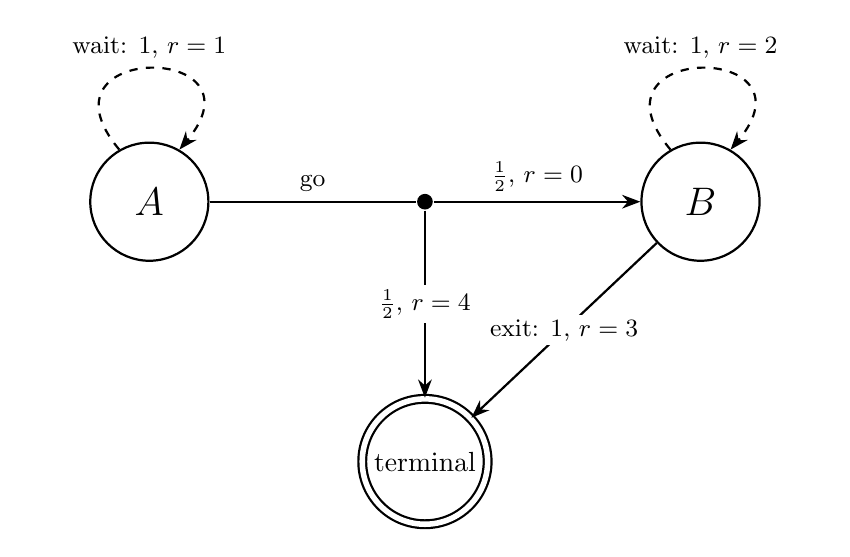
\begin{tikzpicture}[>=Stealth, thick, font=\small,
    st/.style={circle, draw, minimum size=1.5cm, font=\Large},
    lbl/.style={fill=white, inner sep=1.5pt}]
  \node[st] (A) at (0,0) {$A$};
  \node[st] (B) at (7,0) {$B$};
  \node[st, double, double distance=2pt, font=\normalsize] (T) at (3.5,-3.3) {terminal};
  \node[circle, fill, inner sep=2pt] (g) at (3.5,0) {};
  % A: wait (deterministic self-loop)
  \draw[->, dashed] (A.120) to[out=130, in=50, looseness=6] node[above] {wait: $1$, $r=1$} (A.60);
  % A: go (random)
  \draw (A) -- node[above] {go} (g);
  \draw[->] (g) -- node[above] {$\tfrac12$, $r=0$} (B);
  \draw[->] (g) -- node[lbl] {$\tfrac12$, $r=4$} (T);
  % B: wait and exit (deterministic)
  \draw[->, dashed] (B.120) to[out=130, in=50, looseness=6] node[above] {wait: $1$, $r=2$} (B.60);
  \draw[->] (B) -- node[lbl] {exit: $1$, $r=3$} (T);
\end{tikzpicture}
\end{center}

The policy $\pi$ chooses wait and go with probability $\tfrac12$ each at $A$, and always chooses exit at $B$. Every
sweep (i.e. an application of a step of an iterative algorithm) below is \textbf{synchronous}: all new entries use the previous sweep's table. Terminal continuation is always
zero.

\begin{parts}
\part[6] Starting from the expected-return meaning of $\vpi$, write the two Bellman equations for this particular
policy. Show where both the policy probability and the transition probability enter at $A$. Explain why the remaining
return after reaching $B$ can be replaced by $\vpi(B)$. Do not solve the equations.
\begin{solution}
\[
\vpi(A)=\tfrac12\big[1+\tfrac12\vpi(A)\big]+\tfrac12\Big\{\tfrac12\big[0+\tfrac12\vpi(B)\big]+\tfrac12\big[4+\tfrac12\cdot 0\big]\Big\},
\qquad \vpi(B)=3 .
\]
Equivalently $\vpi(A)=\tfrac32+\tfrac14\vpi(A)+\tfrac18\vpi(B)$. The outer $\tfrac12$'s are $\pi(a\mid A)$; the inner
$\tfrac12$'s are the outcome probabilities of go. Given the next state $B$, the Markov property and continued use of
$\pi$ make the expected remaining return $\vpi(B)$.
Rubric: policy averaging 1, wait reward and continuation 1, averaging over go's outcomes 1, go's reward, discount
and terminal handling 1, $B$ equation 1, conditional-return explanation 1. (Exact solution, not required: $(5/2, 3)$.)
\end{solution}
\vfill
\newpage

\part[4] Starting with $V_0(A)=V_0(B)=0$, perform two synchronous policy-evaluation sweeps for $\pi$. Fill in the
table, showing each backup.

\begin{center}
\renewcommand{\arraystretch}{1.2}
\begin{tabular}{|c|c|c|}
\hline
$k$ & $V_k(A)$ & $V_k(B)$ \\ \hline
0 & 0 & 0 \\ \hline
1\cell & \myAnswer{$3/2$} & \myAnswer{$3$} \\ \hline
2\cell & \myAnswer{$9/4$} & \myAnswer{$3$} \\ \hline
\end{tabular}
\end{center}
\begin{solution}
$V_1(A)=\tfrac12(1+0)+\tfrac12\big(\tfrac12\cdot 0+\tfrac12\cdot 4\big)=\tfrac32$, $V_1(B)=3$.
$V_2(A)=\tfrac32+\tfrac14 V_1(A)+\tfrac18 V_1(B)=\tfrac32+\tfrac38+\tfrac38=\tfrac94$, $V_2(B)=3$.
Rubric: 1 per cell (backup from the previous table 0.5, result 0.5). Carry a student's own earlier values forward;
in-place updates keep the method credit but lose the affected result credit.
\end{solution}
\vfill
\newpage

\part[8] Start again from $V_0(A)=V_0(B)=0$. Perform two synchronous \textbf{value-iteration} sweeps, showing both
action-backup values at each state and identifying the maximum. Do not continue the table from part (b).

\begin{center}
\renewcommand{\arraystretch}{1.2}
\begin{tabular}{|c|c|c|c|c|c|c|}
\hline
Sweep & $A$: wait & $A$: go & $V(A)$ & $B$: wait & $B$: exit & $V(B)$ \\ \hline
1\cell & \myAnswer{1} & \myAnswer{2} & \myAnswer{2} & \myAnswer{2} & \myAnswer{3} & \myAnswer{3} \\ \hline
2\cell & \myAnswer{2} & \myAnswer{$11/4$} & \myAnswer{$11/4$} & \myAnswer{$7/2$} & \myAnswer{3} & \myAnswer{$7/2$} \\ \hline
\end{tabular}
\end{center}
\begin{solution}
Sweep 2 from $(2,3)$: $A$ wait $1+\tfrac12\cdot 2=2$; $A$ go $\tfrac12\big(0+\tfrac12\cdot 3\big)+\tfrac12\cdot 4=\tfrac{11}{4}$;
$B$ wait $2+\tfrac12\cdot 3=\tfrac72$; $B$ exit $3$. The maximizing action at $B$ changes from exit to wait.
Rubric: for each state and sweep, both action backups 1 (0.5 each) and the maximum 1; four rows, 8 in total.
\end{solution}
\vfill

\part[8] Independently of parts (b) and (c), the exact values of the original policy are supplied:
$\vpi(A)=\tfrac52$ and $\vpi(B)=3$. Compute $\qpi$ for each of the four state--action pairs. State the greedy improved
policy and check that its selected $\qpi$ value is at least $\vpi$ at each state.
\begin{solution}
$\qpi(A,\text{wait})=1+\tfrac12\cdot\tfrac52=\tfrac94$; $\qpi(A,\text{go})=\tfrac12\big(0+\tfrac12\cdot 3\big)+\tfrac12\cdot 4=\tfrac{11}{4}$;
$\qpi(B,\text{wait})=2+\tfrac12\cdot 3=\tfrac72$; $\qpi(B,\text{exit})=3$ (1 each).
Greedy policy: go at $A$, wait at $B$ (1 each). Checks: $\tfrac{11}{4}\ge\tfrac52$ and $\tfrac72\ge 3$ (1 each). These
are action values under the original $\pi$ after the first action, not the values of the new policy; do not label
them $v^*$.
\end{solution}
\vfill
\newpage

\part[6] Let $\pi'$ be the greedy policy from part (d). Part (d) checks that using $\pi'$ for one step and then
following $\pi$ is at least as good as following $\pi$ throughout: $\vpi(s)\le\qpi(s,\pi'(s))$ at both states. Explain why
using $\pi'$ for two steps and then following $\pi$ is at least as good as using it for one step. (Hint: apply the same
inequality at the state reached after the first step.) What happens as the number of steps using $\pi'$ grows, and what
does this imply about $v^{\pi'}$ and $\vpi$? Then state the main difference between a policy-iteration cycle and a
value-iteration sweep.
\begin{solution}
$\qpi(s,\pi'(s))$ is the expected value of $R_{t+1}+\gamma\vpi(S_{t+1})$ when $\pi'(s)$ is taken. Replacing $\vpi(S_{t+1})$
by $\qpi(S_{t+1},\pi'(S_{t+1}))$ lowers no term (at a terminal successor both continuations are zero), and probabilities and
$\gamma$ are nonnegative, so the average does not fall; the result is two steps of $\pi'$ and then $\pi$. Repeating gives
$k$ steps of $\pi'$ followed by $\pi$, a sequence that never decreases. Values are bounded and the remaining part is
discounted by $\gamma^k\to 0$, so the limit is $v^{\pi'}$ and $v^{\pi'}(s)\ge\vpi(s)$. Here $A$: $\tfrac52,\tfrac{11}{4},\tfrac{23}{8},\ldots\to 3$
and $B$: $3,\tfrac72,\tfrac{15}{4},\ldots\to 4$ (not required).
Policy iteration evaluates a fixed policy (exactly or nearly) and then improves it greedily; value iteration applies
the maximizing backup in every sweep without first completing a fixed-policy evaluation.
Rubric: two-step argument 2 (inequality at each successor 1, averaging preserves it 1), growing $k$ 1, vanishing tail
and conclusion 1, PI 1, VI 1. Accept a verbal argument. Award the reasoning points independently of a mistaken action
choice in (d) when the student correctly uses the supplied inequality.
\end{solution}
\vfill
\newpage

%%%%%%%%%%%%%%%%%%%%%%%%%%%%%%%%%%%%%%%%%%%%%%%%%%%%%%%%%%%%%%%%%%%%%%%%%%%%%%%%%%%%%
% Q4 (ChatGPT Q3a-b with C02 and the added every-visit estimate (D01); Claude Q3e batch part (D03))
\end{parts}
\question (20 points) A fixed policy $\pi$ produced these two complete episodes. Each arrow is labelled by the reward
received on that transition. The model is unknown. Discount $\gamma = \tfrac12$.

\begin{itemize}
  \item Episode 1: $A \xrightarrow{\;0\;} A \xrightarrow{\;2\;} B \xrightarrow{\;4\;}$ terminal
  \item Episode 2: $A \xrightarrow{\;0\;} B \xrightarrow{\;2\;}$ terminal
\end{itemize}
The actions are omitted because this question only evaluates $\pi$.

\begin{parts}
\part[7] Use \textbf{first-visit} Monte Carlo sample averages over both episodes to estimate $V(A)$ and $V(B)$. Then
give the \textbf{every-visit} Monte Carlo estimate of $V(A)$. For each estimate, list the returns you included.
\begin{solution}
Episode 1 returns: $G_2=4$, $G_1=2+\tfrac12\cdot 4=4$, $G_0=0+\tfrac12\cdot 4=2$. Episode 2: $G_1=2$, $G_0=1$.
First-visit: $V(A)=(2+1)/2=\tfrac32$, $V(B)=(4+2)/2=3$. Every-visit: $V(A)=(2+4+1)/3=\tfrac73$ (episode 1's second
visit to $A$ has return 4).
Rubric: first-visit included returns 2, first-visit estimates 2, every-visit included returns for $A$ 1, its estimate
1, correct visit counts 1.
\end{solution}
\vfill

\part[7] Independently of part (a), initialize $V(A)=2$ and $V(B)=0$. With $\alpha=\tfrac12$, apply TD(0) updates
online, in time order, through \textbf{episode 1 only}. For each transition, give the target and the updated value.

\begin{center}
\renewcommand{\arraystretch}{1.2}
\begin{tabular}{|c|c|c|c|}
\hline
Transition & Target $U_t$ & Updated entry & $(V(A), V(B))$ after \\ \hline
$A \xrightarrow{0} A$\cell & \myAnswer{$0+\tfrac12\cdot 2=1$} & \myAnswer{$V(A)=2+\tfrac12(1-2)=\tfrac32$} & \myAnswer{$(\tfrac32, 0)$} \\ \hline
$A \xrightarrow{2} B$\cell & \myAnswer{$2+\tfrac12\cdot 0=2$} & \myAnswer{$V(A)=\tfrac32+\tfrac12(2-\tfrac32)=\tfrac74$} & \myAnswer{$(\tfrac74, 0)$} \\ \hline
$B \xrightarrow{4}$ terminal\cell & \myAnswer{$4$} & \myAnswer{$V(B)=0+\tfrac12(4-0)=2$} & \myAnswer{$(\tfrac74, 2)$} \\ \hline
\end{tabular}
\end{center}
\begin{solution}
The first target and the subtracted estimate both use the pre-update value $V(A)=2$ (self-transition).
Rubric: each target 1, each update from the student's current table 1, chronological use of the reset table 1.
\end{solution}
\vfill
\newpage

\part[6] This part uses \textbf{new data} and $\gamma = 1$. The data are four complete episodes:
\begin{itemize}
  \item twice: $C \xrightarrow{\;+1\;} D \xrightarrow{\;0\;}$ terminal;
  \item twice: $D \xrightarrow{\;+2\;}$ terminal.
\end{itemize}
Using the batch convention from class (repeated passes over this fixed data, increments summed over a pass with the
table held fixed, and a small enough step size to converge), what do batch Monte Carlo and batch TD(0) converge to for
$V(C)$ and $V(D)$? Which answer would you trust if you knew the process was Markov, and why might you doubt that here?
\begin{solution}
Both methods: $V(D)=(0+0+2+2)/4=1$ (1). Batch MC: $V(C)=1$, the mean of its observed returns (1). Batch TD:
$V(C)=1+V(D)=2$ (2). If the process is Markov, TD's answer uses all four outcomes observed from $D$
(certainty equivalence) (1). Here $D$ gave 0 every time it followed $C$ and 2 every time it started an episode, which
hints that ``$D$'' may hide relevant history; then pooling its outcomes can mislead. Two episodes of each kind are
little evidence either way (1). For the ``trust'' point, also credit a reasoned answer that neither estimate is
guaranteed to be more accurate from four episodes. Do not require a claim that the data prove the process is not
Markov.
\end{solution}
\vfill
\newpage

%%%%%%%%%%%%%%%%%%%%%%%%%%%%%%%%%%%%%%%%%%%%%%%%%%%%%%%%%%%%%%%%%%%%%%%%%%%%%%%%%%%%%
% Q5 (ChatGPT Q4)
\end{parts}
\question (14 points) This is a new independent episode, with $\gamma=\tfrac12$ and time indices $0,1,2,3$:
\[
A \xrightarrow{\;2\;} B \xrightarrow{\;0\;} C \xrightarrow{\;4\;} \text{terminal}.
\]
Hold the value table fixed throughout: $V(A)=0$, $V(B)=4$, $V(C)=6$, and terminal value 0. Targets are for the visit
to $A$ at time 0; do not update the table between calculations.

\begin{parts}
\part[4] Expand the return recursion twice and replace the unobserved return after the second transition with its
value estimate. Write the resulting two-step target $G_{0:2}$ symbolically before inserting numbers.
\begin{solution}
$G_0=R_1+\gamma G_1=R_1+\gamma R_2+\gamma^2 G_2$; replacing $G_2$ with $V(S_2)$ gives
$G_{0:2}=R_1+\gamma R_2+\gamma^2 V(S_2)$.
Rubric: first expansion 1, second expansion with correct discount powers 1, replacement at the second successor 1,
correct target 1.
\end{solution}
\vfill

\part[6] Calculate the one-step target $G_{0:1}$, the two-step target $G_{0:2}$ and the full return $G_0$. For the
full return, indicate why there is no additional bootstrap term.
\begin{solution}
$G_{0:1}=2+\tfrac12\cdot 4=4$. $G_{0:2}=2+\tfrac12\cdot 0+\tfrac14\cdot 6=\tfrac72$.
$G_0=2+\tfrac12\cdot 0+\tfrac14\cdot 4=3$: the episode ended, so there is no continuation to bootstrap from.
Rubric: each target, expression 1 and result 1.
\end{solution}
\vfill
\newpage

\part[1] If this episode arrives one transition at a time, at which time index does the two-step target for $A$ first
become available? Must the learner wait until termination here?
\begin{solution}
At time 2, after observing $R_2=0$ and $S_2=C$; no need to wait for termination at time 3.
\end{solution}
\vfill

\part[3] A student sets $\lambda=1$ in the finite episodic forward $\lambda$-return to remove bootstrapping, then
concludes that the target must be more accurate than TD(0). Assess both claims briefly.
\begin{solution}
At $\lambda=1$ the $\lambda$-return is the complete return and does not bootstrap (1). The accuracy claim is false (1):
removing the table from the target does not remove sampling variability, so the error need not be lower and a good
bootstrapped estimate can help (1).
\end{solution}
\vfill
\end{parts}

%%%%%%%%%%%%%%%%%%%%%%%%%%%%%%%%%%%%%%%%%%%%%%%%%%%%%%%%%%%%%%%%%%%%%%%%%%%%%%%%%%%%%
% Equation sheet (ChatGPT's sheet with C03 (i)-(ii); finite lambda-return included under X1)
\newpage
Several Equations (semantics and context are not given on purpose)

\begin{align*}
G_t &= \sum_{k=0}^{T-t-1}\gamma^{k}R_{t+k+1}, \qquad G_t = R_{t+1}+\gamma G_{t+1}, \qquad G_T = 0 \\[4pt]
\vpi(s) &= \E_\pi[G_t\mid S_t=s], \qquad \qpi(s,a) = \E_\pi[G_t\mid S_t=s, A_t=a] \\[4pt]
\vpi(s) &= \sum_a \pi(a\mid s)\,\qpi(s,a) \\[4pt]
\qpi(s,a) &= \sum_{s',r}\M(s,a,r,s')\big[r+\gamma\,\vpi(s')\big] \\[4pt]
v^*(s) &= \max_a \sum_{s',r}\M(s,a,r,s')\big[r+\gamma\,v^*(s')\big], \qquad \pi^*(s)\in\argmax_a q^*(s,a) \\[4pt]
V_{k+1}(s) &= \sum_a \pi(a\mid s)\sum_{s',r}\M(s,a,r,s')\big[r+\gamma\,V_k(s')\big] \\[4pt]
V_{k+1}(s) &= \max_a \sum_{s',r}\M(s,a,r,s')\big[r+\gamma\,V_k(s')\big] \\[4pt]
V(S_t) &\leftarrow V(S_t)+\alpha\big[U_t-V(S_t)\big] \\[4pt]
U_t &= G_t, \qquad U_t = R_{t+1}+\gamma V(S_{t+1}) \\[4pt]
V(s) &\leftarrow V(s)+\frac{1}{N(s)}\big[G_t-V(s)\big], \qquad S_t=s \\[4pt]
G_t^{\lambda} &= (1-\lambda)\sum_{n=1}^{T-t-1}\lambda^{n-1}G_{t:t+n}+\lambda^{T-t-1}G_t, \qquad 0\le\lambda\le 1,\quad t<T
\end{align*}

\end{questions}

\end{document}
"
%
% Exam Template for UMTYMP and Math Department courses
%
% Using Philip Hirschhorn's exam.cls: http://www-math.mit.edu/~psh/#ExamCls
%
% run pdflatex on a finished exam at least three times to do the grading table on front page.
%
%%%%%%%%%%%%%%%%%%%%%%%%%%%%%%%%%%%%%%%%%%%%%%%%%%%%%%%%%%%%%%%%%%%%%%%%%%%%%%%%%%%%%%%%%%%%%%

\documentclass[11pt]{exam}
\RequirePackage{amssymb, amsfonts, amsmath, latexsym, verbatim, xspace, setspace}
\RequirePackage{tikz, pgflibraryplotmarks}
\usetikzlibrary{arrows.meta}

\usepackage[margin=2.1cm]{geometry}
\usepackage[utf8]{inputenc}
\usepackage[english]{babel}
\usepackage{wrapfig}
\usepackage{textpos}
\usepackage{tabularx}
\usepackage{color}
\usepackage{ulem}
\usepackage{multirow}
\usepackage{enumitem}
\usepackage{multicol}
\usepackage{graphicx}
\usepackage{subcaption}
\usepackage{bbm}
\usepackage[T1]{fontenc}
\usepackage{changepage}

\usepackage{amsmath}
\DeclareMathOperator*{\argmax}{arg\,max}
\DeclareMathOperator*{\argmin}{arg\,min}

\definecolor{red}{rgb}{1.0,0.0,0.0}
\definecolor{green}{rgb}{0.0,1.0,0.0}
\definecolor{blue}{rgb}{0.0,0.0,1.0}

\newif\ifexternal
%\externaltrue

\newif\ifonline
\onlinefalse

% Answers are printed only when \withsolutions is defined (see the build lines at the top).
\ifdefined\withsolutions \printanswers \fi
\newcommand{\myAnswer}[1]{\ifprintanswers {\color{blue}#1} \fi}
\newcommand{\myAB}[2]{\ifprintanswers {\color{blue}#1} \else #1 \fi}
\newcommand{\myBlank}[1]{\ifprintanswers {\color{blue}#1} \else \hphantom{#1} \fi}

\SolutionEmphasis{\color{blue}}
\unframedsolutions

% Here's where you edit the Class, Exam, Date, etc.
\newcommand{\class}{COMP 438/538}
\newcommand{\classname}{COMP 438/538: INTRODUCTION TO REINFORCEMENT LEARNING}
\newcommand{\term}{Fall 2026}
\newcommand{\examnum}{MT1}
\newcommand{\examname}{Midterm 1}

\newcommand{\examdate}{05/11/2026}
\newcommand{\timelimit}{100 Minutes}
\newcommand{\instructor}{Bar\i\c{s} Akg\"un}

% Course notation (course/notation_guide.md)
\newcommand{\M}{\mathcal{M}}
\newcommand{\E}{\mathbb{E}}
\newcommand{\vpi}{v^{\pi}}
\newcommand{\qpi}{q^{\pi}}
\newcommand{\cell}{\rule{0pt}{1.1cm}}

\parindent 0ex

\newcolumntype{L}{>{\raggedright\arraybackslash}X}%
\newcolumntype{R}{>{\raggedleft\arraybackslash}X}%
\newcolumntype{C}{>{\centering\arraybackslash}X}

\setlength{\abovedisplayskip}{4pt}
\setlength{\belowdisplayskip}{4pt}
\setlength{\abovedisplayshortskip}{2pt}
\setlength{\belowdisplayshortskip}{2pt}

\begin{document}

  \begin{center}
    {\scshape\Large KO\c{C} UNIVERSITY \par}
    {\scshape\Large College of Engineering\par}
    \vspace{0.5cm}
    {\LARGE\bfseries \classname \par}
    \vspace{0.5cm}
    {\scshape\Large \bfseries \examname \par}
    {\scshape\large \term, \examdate \par}
    {\scshape\large Duration: \timelimit  \par}
    \vspace{0.3cm}
    \hrulefill
    \vspace{0.2cm}
  \end{center}

    \begin{tabular}{l l}
      \textbf{Name:} & \makebox[10cm]{\uline{ \myAnswer{Solutions} \hfill }}   \\
      & \\
      \textbf{ID:} & \makebox[10cm]{\uline{ \myAnswer{00110001 00110000 00110000} \hfill }}
    \end{tabular}

  \vspace{0.4cm}
  \hrulefill
\begin{center}
{\large \bfseries Read These Instructions Carefully}
\end{center}
\begin{itemize}
  \item This exam contains \numpages\ pages including this cover page and \numquestions\ questions. Check to see if any
  pages are missing. Put your initials on the top of every page, in case the pages become separated.
  \item  By submitting this exam, you \textbf{agree} to fully comply with Ko\c{c} University Student Code of Conduct,
  and accept any punishment in case of failure to comply. If you do not submit this exam on time, you will receive 0 credits.
  \item The exam is \textbf{closed book} and \textbf{closed notes}. You are \textbf{not} allowed to use any additional
  material including any electronic equipment such as computers and  mobile phones. An equation sheet is provided on
  the last page.
  \item You are expected to be able to provide clear and concise answers. Gibberish will not receive any credit. Your answers need to be readable by a human,
  illegible writing is not gradable.
  \item Show the essential calculations or a short justification. Exact fractions or equivalent decimals are acceptable.
  Each question describes a separate problem; state names are local to their question. Terminal states have zero
  continuation value, and a reward shown on a transition is the total reward for that transition.
  \item Read each question \uline{carefully} and make sure to follow instructions. The written instructions take
  precedence over an answer that the instructor might give you during the exam, unless the instructor makes a class-wide announcement.
  \item Do not write in the table below.
\end{itemize}

\hrulefill
  \begin{center}
    \vspace{0.2cm}
    \gradetablestretch{1.8}
    \vqword{Question}
    \addpoints
    \gradetable[h]
  \end{center}

\newpage % End of cover page
\runningheader{\class}{\examnum\ - Page \thepage\ of \numpages}{\examdate}
\runningheadrule

\begin{questions}

%%%%%%%%%%%%%%%%%%%%%%%%%%%%%%%%%%%%%%%%%%%%%%%%%%%%%%%%%%%%%%%%%%%%%%%%%%%%%%%%%%%%%
% Q1: short answers, placed first as a warm-up (instructor, 2026-11-03). Was Q5: ChatGPT Q5a, Q5b (X8);
% Claude T/F 3 true form, 4, 5.
\question (12 points) Short answers.

\begin{parts}
\part[2] Consider two policies for a continuing service task. One produces reward 0.75 every step. The other repeats
the rewards $0, 2, 0, 2, \ldots$ forever. Which has the higher long-run average reward per step, and why? No
average-reward learning algorithm is required.
\begin{solution}
The alternating policy: $(0+2)/2=1$ per step versus 0.75 (1 for the rates, 1 for the comparison).
\end{solution}
\vfill

\part[4] A report compares MC and TD prediction on a fixed policy. It tries many step sizes and selects each method's
best setting using the same episodes and seeds on which it reports final value error. It then uses the single
lowest-error run to claim that the selected method is generally better. Identify two weaknesses and suggest a fix for each. 
No statistical test or numerical uncertainty calculation is required.
\begin{solution}
(1) Settings were chosen on the runs used for the reported result, so the result is optimistic; repair: choose
settings on separate development runs, then report fresh final runs at those settings. (2) One best run does not show
typical performance; repair: run many independent runs and report the mean error with its variability, not the best
seed. Rubric: 1 per weakness, 1 per repair. A fair-budget answer earns credit only if it is tied to one of these flaws.
\end{solution}
\vfill
\newpage

\uplevel{For each statement below, write \textbf{True} or \textbf{False} and give a one-line justification. Each is
worth 2 points: 1 for the verdict and 1 for the justification. A verdict without a justification receives 0.}

\part[2] Given $q^*$, a greedy optimal policy can be obtained without the model, however, obtaining one from $v^*$ by one-step
lookahead needs the model.
\begin{solution}
True: $\argmax_a q^*(s,a)$ needs no model; with $v^*$, comparing actions needs the expected rewards and transition
probabilities.
\end{solution}
\vfill

\part[2] If the current policy is not optimal, one greedy policy-improvement step using its exact action values
increases the value of at least one nonterminal state.
\begin{solution}
True: a suboptimal policy must admit a strict one-step gain somewhere; otherwise $\vpi(s)=\max_a\qpi(s,a)$ at every
state, which is the Bellman optimality equation. By the policy improvement theorem the greedy policy keeps that gain
and lowers no state. Rubric: verdict 1, reason for the strict gain 1, in ordinary language. Naming the policy
improvement theorem without that reason earns 0.5 of the reason point; a change of action at a tie alone earns none.
\end{solution}
\vfill

\part[2] The Monte Carlo prediction method we used in class can be applied directly to a continuing task that never
terminates.
\begin{solution}
False: the method waits for a finished episode to observe its target, so without termination it never gets one.
Rubric: verdict 1, reason 1. Full credit for explaining that a finite cutoff would change the target; ``True, by
truncating'' earns no verdict point. Mentioning TD is not required.
\end{solution}
\vfill

\end{parts}
\newpage

%%%%%%%%%%%%%%%%%%%%%%%%%%%%%%%%%%%%%%%%%%%%%%%%%%%%%%%%%%%%%%%%%%%%%%%%%%%%%%%%%%%%%
% Q2 (Claude Q1 with review wording R01-R03). Partial credit for alternative answers: instructor (X6).
\question (22 points) An online tutoring app runs a practice session of exactly 20 questions. Before each question it
chooses a difficulty: easy, medium or hard. After each question it sees only whether the answer was correct and how
many seconds it took. The student's actual skill is not visible, and it changes as the student practises. After the
20th question the student takes a fixed 10-question test that the app does not choose.

The designer's objective is to maximize the student's expected score on the fixed final test. No model of how
difficulty affects skill, correctness or response time is supplied.

\begin{parts}
\part[4] What are the actions? What does the app observe after each question?
\begin{solution}
Actions: easy, medium, hard (2). Observation after each question: whether the answer was correct and the response
time (2). Additional observed features (e.g.\ the topic) are fine if justified.
\end{solution}
\vfill

\part[6] Explain why the latest observation alone need not be a Markov state. Give two plausible histories ending in
the same observation that could suggest different skill levels. Propose a history-based agent state for choosing the
next difficulty, justify the information you retain, and mention one limitation. A justified approximation is
sufficient; you do not need to prove that it is Markov.
\begin{solution}
The skill is hidden and changes, so the latest answer alone does not summarize what matters for the next outcome (1).
Example: ``correct, 20 seconds'' after ten correct hard answers versus after ten wrong easy answers suggests very
different skill and a different next difficulty (2). Example agent state $S_t = f(H_t)$: recent counts of correct
answers per difficulty (or an estimated skill level), plus questions remaining (2). Justification and one limitation,
e.g.\ counts discard the order of answers, so improvement over the session can be missed (1).
\end{solution}
\vfill
\newpage

\part[6] Designer A rewards each correct practice answer with $+1$ and gives $0$ otherwise. Designer B gives the final
test score ($0$--$10$) after the session and $0$ otherwise. Describe a plausible way A could encourage behaviour that
does not improve the final test score. Which reward more directly matches the stated objective, and what makes
learning from it difficult? You do not need to identify an optimal sequence of difficulties.
\begin{solution}
A can encourage choosing easy questions for immediate correct answers even when harder practice would teach more: an
incentive mismatch, not a claim about the optimal policy for every student (2). B rewards the stated objective
directly (2), but the feedback is delayed and sparse: one number after 20 decisions, so assigning credit to
individual difficulty choices is hard and many sessions are needed (2).
\end{solution}
\vfill

\part[4] Is the task episodic or continuing? Should the number of questions remaining be part of the agent state? Why?
\begin{solution}
Episodic: the session ends after 20 questions and the test (1). Yes (1): with a deadline, the best difficulty can
depend on the time left, e.g.\ hard practice may pay off only if enough practice follows, so the same skill estimate
with 2 or 15 questions left can call for different actions (2). The ``Yes'' point does not require a separate
counter: a state that already contains the remaining number of questions, e.g.\ the full history or the elapsed
number of questions, earns it.
\end{solution}
\vfill

\part[2] With no model of the student's responses or learning dynamics supplied, can you directly apply ordinary
tabular value iteration to compute a policy? What information would be needed?
\begin{solution}
No (1): value iteration needs the expected rewards and next-state probabilities for a usable Markov state, which are
not provided; experience, or an independently supplied model, would be needed (1). A conditional answer (``with a
usable Markov model, yes'') earns full credit.
\end{solution}
\vfill
\newpage

%%%%%%%%%%%%%%%%%%%%%%%%%%%%%%%%%%%%%%%%%%%%%%%%%%%%%%%%%%%%%%%%%%%%%%%%%%%%%%%%%%%%%
% Q3 (ChatGPT Q2; Q3b 4 points under X8; model figure replaces the table, instructor 2026-11-03)
\end{parts}
\question (32 points) There are two nonterminal states $A$ and $B$, and a terminal state. The discount is
$\gamma = \tfrac12$. The figure shows every possible transition. The black dot shows the possible outcomes after choosing go. Each arrow
gives the probability $\M(s,a,r,s')$ and the reward $r$ of its outcome. All other outcomes have probability zero.

\begin{center}
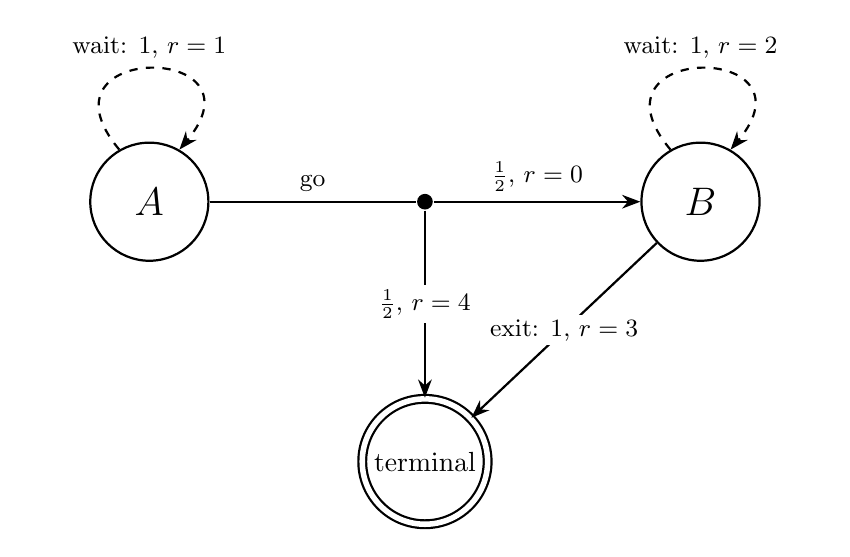
\begin{tikzpicture}[>=Stealth, thick, font=\small,
    st/.style={circle, draw, minimum size=1.5cm, font=\Large},
    lbl/.style={fill=white, inner sep=1.5pt}]
  \node[st] (A) at (0,0) {$A$};
  \node[st] (B) at (7,0) {$B$};
  \node[st, double, double distance=2pt, font=\normalsize] (T) at (3.5,-3.3) {terminal};
  \node[circle, fill, inner sep=2pt] (g) at (3.5,0) {};
  % A: wait (deterministic self-loop)
  \draw[->, dashed] (A.120) to[out=130, in=50, looseness=6] node[above] {wait: $1$, $r=1$} (A.60);
  % A: go (random)
  \draw (A) -- node[above] {go} (g);
  \draw[->] (g) -- node[above] {$\tfrac12$, $r=0$} (B);
  \draw[->] (g) -- node[lbl] {$\tfrac12$, $r=4$} (T);
  % B: wait and exit (deterministic)
  \draw[->, dashed] (B.120) to[out=130, in=50, looseness=6] node[above] {wait: $1$, $r=2$} (B.60);
  \draw[->] (B) -- node[lbl] {exit: $1$, $r=3$} (T);
\end{tikzpicture}
\end{center}

The policy $\pi$ chooses wait and go with probability $\tfrac12$ each at $A$, and always chooses exit at $B$. Every
sweep (i.e. an application of a step of an iterative algorithm) below is \textbf{synchronous}: all new entries use the previous sweep's table. Terminal continuation is always
zero.

\begin{parts}
\part[6] Starting from the expected-return meaning of $\vpi$, write the two Bellman equations for this particular
policy. Show where both the policy probability and the transition probability enter at $A$. Explain why the remaining
return after reaching $B$ can be replaced by $\vpi(B)$. Do not solve the equations.
\begin{solution}
\[
\vpi(A)=\tfrac12\big[1+\tfrac12\vpi(A)\big]+\tfrac12\Big\{\tfrac12\big[0+\tfrac12\vpi(B)\big]+\tfrac12\big[4+\tfrac12\cdot 0\big]\Big\},
\qquad \vpi(B)=3 .
\]
Equivalently $\vpi(A)=\tfrac32+\tfrac14\vpi(A)+\tfrac18\vpi(B)$. The outer $\tfrac12$'s are $\pi(a\mid A)$; the inner
$\tfrac12$'s are the outcome probabilities of go. Given the next state $B$, the Markov property and continued use of
$\pi$ make the expected remaining return $\vpi(B)$.
Rubric: policy averaging 1, wait reward and continuation 1, averaging over go's outcomes 1, go's reward, discount
and terminal handling 1, $B$ equation 1, conditional-return explanation 1. (Exact solution, not required: $(5/2, 3)$.)
\end{solution}
\vfill
\newpage

\part[4] Starting with $V_0(A)=V_0(B)=0$, perform two synchronous policy-evaluation sweeps for $\pi$. Fill in the
table, showing each backup.

\begin{center}
\renewcommand{\arraystretch}{1.2}
\begin{tabular}{|c|c|c|}
\hline
$k$ & $V_k(A)$ & $V_k(B)$ \\ \hline
0 & 0 & 0 \\ \hline
1\cell & \myAnswer{$3/2$} & \myAnswer{$3$} \\ \hline
2\cell & \myAnswer{$9/4$} & \myAnswer{$3$} \\ \hline
\end{tabular}
\end{center}
\begin{solution}
$V_1(A)=\tfrac12(1+0)+\tfrac12\big(\tfrac12\cdot 0+\tfrac12\cdot 4\big)=\tfrac32$, $V_1(B)=3$.
$V_2(A)=\tfrac32+\tfrac14 V_1(A)+\tfrac18 V_1(B)=\tfrac32+\tfrac38+\tfrac38=\tfrac94$, $V_2(B)=3$.
Rubric: 1 per cell (backup from the previous table 0.5, result 0.5). Carry a student's own earlier values forward;
in-place updates keep the method credit but lose the affected result credit.
\end{solution}
\vfill
\newpage

\part[8] Start again from $V_0(A)=V_0(B)=0$. Perform two synchronous \textbf{value-iteration} sweeps, showing both
action-backup values at each state and identifying the maximum. Do not continue the table from part (b).

\begin{center}
\renewcommand{\arraystretch}{1.2}
\begin{tabular}{|c|c|c|c|c|c|c|}
\hline
Sweep & $A$: wait & $A$: go & $V(A)$ & $B$: wait & $B$: exit & $V(B)$ \\ \hline
1\cell & \myAnswer{1} & \myAnswer{2} & \myAnswer{2} & \myAnswer{2} & \myAnswer{3} & \myAnswer{3} \\ \hline
2\cell & \myAnswer{2} & \myAnswer{$11/4$} & \myAnswer{$11/4$} & \myAnswer{$7/2$} & \myAnswer{3} & \myAnswer{$7/2$} \\ \hline
\end{tabular}
\end{center}
\begin{solution}
Sweep 2 from $(2,3)$: $A$ wait $1+\tfrac12\cdot 2=2$; $A$ go $\tfrac12\big(0+\tfrac12\cdot 3\big)+\tfrac12\cdot 4=\tfrac{11}{4}$;
$B$ wait $2+\tfrac12\cdot 3=\tfrac72$; $B$ exit $3$. The maximizing action at $B$ changes from exit to wait.
Rubric: for each state and sweep, both action backups 1 (0.5 each) and the maximum 1; four rows, 8 in total.
\end{solution}
\vfill

\part[8] Independently of parts (b) and (c), the exact values of the original policy are supplied:
$\vpi(A)=\tfrac52$ and $\vpi(B)=3$. Compute $\qpi$ for each of the four state--action pairs. State the greedy improved
policy and check that its selected $\qpi$ value is at least $\vpi$ at each state.
\begin{solution}
$\qpi(A,\text{wait})=1+\tfrac12\cdot\tfrac52=\tfrac94$; $\qpi(A,\text{go})=\tfrac12\big(0+\tfrac12\cdot 3\big)+\tfrac12\cdot 4=\tfrac{11}{4}$;
$\qpi(B,\text{wait})=2+\tfrac12\cdot 3=\tfrac72$; $\qpi(B,\text{exit})=3$ (1 each).
Greedy policy: go at $A$, wait at $B$ (1 each). Checks: $\tfrac{11}{4}\ge\tfrac52$ and $\tfrac72\ge 3$ (1 each). These
are action values under the original $\pi$ after the first action, not the values of the new policy; do not label
them $v^*$.
\end{solution}
\vfill
\newpage

\part[6] Let $\pi'$ be the greedy policy from part (d). Part (d) checks that using $\pi'$ for one step and then
following $\pi$ is at least as good as following $\pi$ throughout: $\vpi(s)\le\qpi(s,\pi'(s))$ at both states. Explain why
using $\pi'$ for two steps and then following $\pi$ is at least as good as using it for one step. (Hint: apply the same
inequality at the state reached after the first step.) What happens as the number of steps using $\pi'$ grows, and what
does this imply about $v^{\pi'}$ and $\vpi$? Then state the main difference between a policy-iteration cycle and a
value-iteration sweep.
\begin{solution}
$\qpi(s,\pi'(s))$ is the expected value of $R_{t+1}+\gamma\vpi(S_{t+1})$ when $\pi'(s)$ is taken. Replacing $\vpi(S_{t+1})$
by $\qpi(S_{t+1},\pi'(S_{t+1}))$ lowers no term (at a terminal successor both continuations are zero), and probabilities and
$\gamma$ are nonnegative, so the average does not fall; the result is two steps of $\pi'$ and then $\pi$. Repeating gives
$k$ steps of $\pi'$ followed by $\pi$, a sequence that never decreases. Values are bounded and the remaining part is
discounted by $\gamma^k\to 0$, so the limit is $v^{\pi'}$ and $v^{\pi'}(s)\ge\vpi(s)$. Here $A$: $\tfrac52,\tfrac{11}{4},\tfrac{23}{8},\ldots\to 3$
and $B$: $3,\tfrac72,\tfrac{15}{4},\ldots\to 4$ (not required).
Policy iteration evaluates a fixed policy (exactly or nearly) and then improves it greedily; value iteration applies
the maximizing backup in every sweep without first completing a fixed-policy evaluation.
Rubric: two-step argument 2 (inequality at each successor 1, averaging preserves it 1), growing $k$ 1, vanishing tail
and conclusion 1, PI 1, VI 1. Accept a verbal argument. Award the reasoning points independently of a mistaken action
choice in (d) when the student correctly uses the supplied inequality.
\end{solution}
\vfill
\newpage

%%%%%%%%%%%%%%%%%%%%%%%%%%%%%%%%%%%%%%%%%%%%%%%%%%%%%%%%%%%%%%%%%%%%%%%%%%%%%%%%%%%%%
% Q4 (ChatGPT Q3a-b with C02 and the added every-visit estimate (D01); Claude Q3e batch part (D03))
\end{parts}
\question (20 points) A fixed policy $\pi$ produced these two complete episodes. Each arrow is labelled by the reward
received on that transition. The model is unknown. Discount $\gamma = \tfrac12$.

\begin{itemize}
  \item Episode 1: $A \xrightarrow{\;0\;} A \xrightarrow{\;2\;} B \xrightarrow{\;4\;}$ terminal
  \item Episode 2: $A \xrightarrow{\;0\;} B \xrightarrow{\;2\;}$ terminal
\end{itemize}
The actions are omitted because this question only evaluates $\pi$.

\begin{parts}
\part[7] Use \textbf{first-visit} Monte Carlo sample averages over both episodes to estimate $V(A)$ and $V(B)$. Then
give the \textbf{every-visit} Monte Carlo estimate of $V(A)$. For each estimate, list the returns you included.
\begin{solution}
Episode 1 returns: $G_2=4$, $G_1=2+\tfrac12\cdot 4=4$, $G_0=0+\tfrac12\cdot 4=2$. Episode 2: $G_1=2$, $G_0=1$.
First-visit: $V(A)=(2+1)/2=\tfrac32$, $V(B)=(4+2)/2=3$. Every-visit: $V(A)=(2+4+1)/3=\tfrac73$ (episode 1's second
visit to $A$ has return 4).
Rubric: first-visit included returns 2, first-visit estimates 2, every-visit included returns for $A$ 1, its estimate
1, correct visit counts 1.
\end{solution}
\vfill

\part[7] Independently of part (a), initialize $V(A)=2$ and $V(B)=0$. With $\alpha=\tfrac12$, apply TD(0) updates
online, in time order, through \textbf{episode 1 only}. For each transition, give the target and the updated value.

\begin{center}
\renewcommand{\arraystretch}{1.2}
\begin{tabular}{|c|c|c|c|}
\hline
Transition & Target $U_t$ & Updated entry & $(V(A), V(B))$ after \\ \hline
$A \xrightarrow{0} A$\cell & \myAnswer{$0+\tfrac12\cdot 2=1$} & \myAnswer{$V(A)=2+\tfrac12(1-2)=\tfrac32$} & \myAnswer{$(\tfrac32, 0)$} \\ \hline
$A \xrightarrow{2} B$\cell & \myAnswer{$2+\tfrac12\cdot 0=2$} & \myAnswer{$V(A)=\tfrac32+\tfrac12(2-\tfrac32)=\tfrac74$} & \myAnswer{$(\tfrac74, 0)$} \\ \hline
$B \xrightarrow{4}$ terminal\cell & \myAnswer{$4$} & \myAnswer{$V(B)=0+\tfrac12(4-0)=2$} & \myAnswer{$(\tfrac74, 2)$} \\ \hline
\end{tabular}
\end{center}
\begin{solution}
The first target and the subtracted estimate both use the pre-update value $V(A)=2$ (self-transition).
Rubric: each target 1, each update from the student's current table 1, chronological use of the reset table 1.
\end{solution}
\vfill
\newpage

\part[6] This part uses \textbf{new data} and $\gamma = 1$. The data are four complete episodes:
\begin{itemize}
  \item twice: $C \xrightarrow{\;+1\;} D \xrightarrow{\;0\;}$ terminal;
  \item twice: $D \xrightarrow{\;+2\;}$ terminal.
\end{itemize}
Using the batch convention from class (repeated passes over this fixed data, increments summed over a pass with the
table held fixed, and a small enough step size to converge), what do batch Monte Carlo and batch TD(0) converge to for
$V(C)$ and $V(D)$? Which answer would you trust if you knew the process was Markov, and why might you doubt that here?
\begin{solution}
Both methods: $V(D)=(0+0+2+2)/4=1$ (1). Batch MC: $V(C)=1$, the mean of its observed returns (1). Batch TD:
$V(C)=1+V(D)=2$ (2). If the process is Markov, TD's answer uses all four outcomes observed from $D$
(certainty equivalence) (1). Here $D$ gave 0 every time it followed $C$ and 2 every time it started an episode, which
hints that ``$D$'' may hide relevant history; then pooling its outcomes can mislead. Two episodes of each kind are
little evidence either way (1). For the ``trust'' point, also credit a reasoned answer that neither estimate is
guaranteed to be more accurate from four episodes. Do not require a claim that the data prove the process is not
Markov.
\end{solution}
\vfill
\newpage

%%%%%%%%%%%%%%%%%%%%%%%%%%%%%%%%%%%%%%%%%%%%%%%%%%%%%%%%%%%%%%%%%%%%%%%%%%%%%%%%%%%%%
% Q5 (ChatGPT Q4)
\end{parts}
\question (14 points) This is a new independent episode, with $\gamma=\tfrac12$ and time indices $0,1,2,3$:
\[
A \xrightarrow{\;2\;} B \xrightarrow{\;0\;} C \xrightarrow{\;4\;} \text{terminal}.
\]
Hold the value table fixed throughout: $V(A)=0$, $V(B)=4$, $V(C)=6$, and terminal value 0. Targets are for the visit
to $A$ at time 0; do not update the table between calculations.

\begin{parts}
\part[4] Expand the return recursion twice and replace the unobserved return after the second transition with its
value estimate. Write the resulting two-step target $G_{0:2}$ symbolically before inserting numbers.
\begin{solution}
$G_0=R_1+\gamma G_1=R_1+\gamma R_2+\gamma^2 G_2$; replacing $G_2$ with $V(S_2)$ gives
$G_{0:2}=R_1+\gamma R_2+\gamma^2 V(S_2)$.
Rubric: first expansion 1, second expansion with correct discount powers 1, replacement at the second successor 1,
correct target 1.
\end{solution}
\vfill

\part[6] Calculate the one-step target $G_{0:1}$, the two-step target $G_{0:2}$ and the full return $G_0$. For the
full return, indicate why there is no additional bootstrap term.
\begin{solution}
$G_{0:1}=2+\tfrac12\cdot 4=4$. $G_{0:2}=2+\tfrac12\cdot 0+\tfrac14\cdot 6=\tfrac72$.
$G_0=2+\tfrac12\cdot 0+\tfrac14\cdot 4=3$: the episode ended, so there is no continuation to bootstrap from.
Rubric: each target, expression 1 and result 1.
\end{solution}
\vfill
\newpage

\part[1] If this episode arrives one transition at a time, at which time index does the two-step target for $A$ first
become available? Must the learner wait until termination here?
\begin{solution}
At time 2, after observing $R_2=0$ and $S_2=C$; no need to wait for termination at time 3.
\end{solution}
\vfill

\part[3] A student sets $\lambda=1$ in the finite episodic forward $\lambda$-return to remove bootstrapping, then
concludes that the target must be more accurate than TD(0). Assess both claims briefly.
\begin{solution}
At $\lambda=1$ the $\lambda$-return is the complete return and does not bootstrap (1). The accuracy claim is false (1):
removing the table from the target does not remove sampling variability, so the error need not be lower and a good
bootstrapped estimate can help (1).
\end{solution}
\vfill
\end{parts}

%%%%%%%%%%%%%%%%%%%%%%%%%%%%%%%%%%%%%%%%%%%%%%%%%%%%%%%%%%%%%%%%%%%%%%%%%%%%%%%%%%%%%
% Equation sheet (ChatGPT's sheet with C03 (i)-(ii); finite lambda-return included under X1)
\newpage
Several Equations (semantics and context are not given on purpose)

\begin{align*}
G_t &= \sum_{k=0}^{T-t-1}\gamma^{k}R_{t+k+1}, \qquad G_t = R_{t+1}+\gamma G_{t+1}, \qquad G_T = 0 \\[4pt]
\vpi(s) &= \E_\pi[G_t\mid S_t=s], \qquad \qpi(s,a) = \E_\pi[G_t\mid S_t=s, A_t=a] \\[4pt]
\vpi(s) &= \sum_a \pi(a\mid s)\,\qpi(s,a) \\[4pt]
\qpi(s,a) &= \sum_{s',r}\M(s,a,r,s')\big[r+\gamma\,\vpi(s')\big] \\[4pt]
v^*(s) &= \max_a \sum_{s',r}\M(s,a,r,s')\big[r+\gamma\,v^*(s')\big], \qquad \pi^*(s)\in\argmax_a q^*(s,a) \\[4pt]
V_{k+1}(s) &= \sum_a \pi(a\mid s)\sum_{s',r}\M(s,a,r,s')\big[r+\gamma\,V_k(s')\big] \\[4pt]
V_{k+1}(s) &= \max_a \sum_{s',r}\M(s,a,r,s')\big[r+\gamma\,V_k(s')\big] \\[4pt]
V(S_t) &\leftarrow V(S_t)+\alpha\big[U_t-V(S_t)\big] \\[4pt]
U_t &= G_t, \qquad U_t = R_{t+1}+\gamma V(S_{t+1}) \\[4pt]
V(s) &\leftarrow V(s)+\frac{1}{N(s)}\big[G_t-V(s)\big], \qquad S_t=s \\[4pt]
G_t^{\lambda} &= (1-\lambda)\sum_{n=1}^{T-t-1}\lambda^{n-1}G_{t:t+n}+\lambda^{T-t-1}G_t, \qquad 0\le\lambda\le 1,\quad t<T
\end{align*}

\end{questions}

\end{document}
